%Version 3.1 December 2024
\documentclass[pdflatex,sn-mathphys-num]{sn-jnl}

\usepackage[utf8]{inputenc}
\usepackage{graphicx}
\usepackage{multirow}
\usepackage{amsmath,amssymb,amsfonts}
\usepackage{amsthm}
\usepackage{mathrsfs}
\usepackage[title]{appendix}
\usepackage{xcolor}
\usepackage{textcomp}
\usepackage{manyfoot}
\usepackage{booktabs}
\usepackage{algorithm}
\usepackage{algorithmicx}
\usepackage{algpseudocode}
\usepackage{listings}
\usepackage{subcaption}

\theoremstyle{thmstyleone}
\newtheorem{theorem}{Theorem}
\newtheorem{proposition}[theorem]{Proposition}
\theoremstyle{thmstyletwo}
\newtheorem{example}{Example}
\newtheorem{remark}{Remark}
\theoremstyle{thmstylethree}
\newtheorem{definition}{Definition}

\raggedbottom

\begin{document}

\title[PREDICT-AML]{PREDICT-AML: Personalized REsponse via Drug Interaction with Cellular Traits for Acute Myeloid Leukemia}

\author[1]{\fnm {Mohammed} \sur{Al-Ani}}\email{moal34112@hbku.edu.qa}
\author[2,3]{\fnm{Siddhi P.} \sur{Jani}}\email{siddhijani@cbr-iisc.ac.in}

\author[4]{\fnm{Halima} \sur{Bensmail}}\email{hbensmail@hbku.edu.qa}

\author[4,5]{\fnm{Raghvendra} \sur{Mall}}\email{raghvendramall@ieee.org}
\equalcont{Corresponding author}

\affil[1]{\orgdiv{College of Health and Life Sciences}, \orgname{Hamad Bin Khalifa University},
\orgaddress{\city{Doha}, \country{Qatar}}}

\affil[2]{\orgdiv{Institute of Science}, \orgname{Nirma University},
\orgaddress{\city{Ahmedabad}, \country{India}}}

\affil[3]{\orgdiv{Centre of Brain Research}, \orgname{Indian Institute of Sciences},
\orgaddress{\city{Bangalore}, \state{Karnataka}, \country{India}}}

\affil[4]{\orgdiv{Qatar Computing Research Institute}, \orgname{Hamad Bin Khalifa University},
\orgaddress{\city{Doha}, \country{Qatar}}}

\affil[5]{\orgdiv{Biotechnology Research Center}, \orgname{Technology Innovation Institute},
\orgaddress{\city{Abu Dhabi}, \postcode{9639}, \country{U.A.E}}}

\abstract{
\textbf{Motivation}: Acute myeloid leukemia (AML) is a biologically heterogeneous hematologic malignancy with limited therapeutic options. The BeatAML cohort profiled specimens from $805$ patients, integrating \textit{ex vivo} drug sensitivity measurements across $165$ drugs with clinical annotations, DNA sequencing, and RNA sequencing. We present PREDICT-AML, a machine learning framework that leverages this resource to generate generalizable, personalized drug response predictions from patients' clinical, genomic, and transcriptomic profiles. \\
\textbf{Methods}: PREDICT-AML employs four complementary drug representations: (a) physicochemical descriptors, (b) knowledge-distilled embeddings (KD-Embed), and chemical language model embeddings from (c) ChemBERTa and (d) MolFormer. These are combined with novel patient-specific oncogenic pathway proximity scores, cell-state enrichments, and genomic profiles. The tabular foundation model, TabPFN, was identified as the optimal architecture following systematic hyperparameter optimization via Optuna. \\
\textbf{Results}: The KD-Embed configuration achieves optimal $r_{pc} = 0.690$ and MAE $= 37.712$ on the held-out BeatAML test set (Waves~3+4). Under patient-stratified cross-validation (PS-CV), a clinically meaningful benchmark, the model achieves $r_{pc} = 0.724 \pm 0.015$, whereas standard random cross-validation inflates this to $r_{pc} = 0.806 \pm 0.001$, overestimating correlation by $\sim\!11\%$. Drug-stratified cross-validation reveals further generalization challenges ($r_{pc} = 0.312 \pm 0.059$). External validation on the LeeAML cohort, evaluating $30$ patients across $49$ drugs overlapping with BeatAML, yielded $r_{pc} = 0.597$. On the FIMM-AML cohort, evaluating $187$ patients across $78$ drugs overlapping with BeatAML, the model achieves $|r_{pc}| = 0.557$, where the sign reflects the opposing directionality of AUC and DSS sensitivity metrics across platforms. \\
\textbf{Availability}: All source code is publicly available at \url{https://github.com/raghvendra5688/PT-AML2.0}.
}

\keywords{Personalized Drug Response, Acute Myeloid Leukemia, Multi-omics Integration, External Validation, TabPFN, Transformers}

\maketitle

%%%%%%%%%%%%%%%%%%%%%%%%%%%%%%%%%%%%%%%%%%%%%
\section{Introduction}\label{sec1}
Acute Myeloid Leukemia (AML) is a biologically and clinically heterogeneous hematologic malignancy characterized by a broad range of genetic mutations, epigenetic alterations, and molecular subtypes \cite{cancer2013genomic,papaemmanuil2016genomic,kurzer2023updates,tyner2018functional}. According to the Surveillance, Epidemiology, and End Results (SEER) program, AML is expected to account for an estimated $22{,}010$ new cases in the United States in 2025, representing approximately $1.1\%$ of all new cancer diagnoses and causing around $11{,}090$ deaths ($2\%$ of all cancer-related fatalities), underscoring its disproportionately high mortality relative to incidence. This clinical burden reflects the urgent need for improved therapeutic strategies and more precise treatment selection. The disease's complexity and variability present significant challenges to conventional treatment approaches, as patients often show diverse responses to standard chemotherapies and targeted agents. Despite progress in drug development, predicting which therapy will be most effective for a given patient remains a formidable clinical challenge \cite{tyner2018functional,yu2020advances}. While recent advances in genomics have led to the development of targeted therapies, accurately predicting individual AML patient response to specific drugs remains a major obstacle \cite{shafiei2025omics}.

In response to the persistent challenge of therapeutic heterogeneity in AML, precision medicine initiatives have gained momentum as a means to tailor treatments based on the unique molecular profiles of individual patients \cite{lohse2018precision}. One of the most significant efforts in this domain is the BeatAML project \cite{tyner2018functional}, a large-scale, multi-institutional initiative led by the Leukemia \& Lymphoma Society. The project emerged from the recognition that traditional one-size-fits-all treatment paradigms are insufficient for a disease as biologically diverse as AML \cite{bottomly2022integrative}. Earlier studies had shown that AML comprises multiple subtypes with distinct genomic and transcriptomic signatures, each of which may respond differently to specific therapies \cite{mo2023integrative,bottomly2022integrative}.

The BeatAML initiative \cite{bottomly2022integrative} sought to address this gap by building a comprehensive, high-resolution resource that integrates multi-omics data including: whole-exome sequencing, RNA sequencing, and clinical annotations together with \textit{ex vivo} drug sensitivity profiling. By systematically collecting and analyzing $942$ patient-derived AML specimens from $805$ individuals, the cohort captures a broad range of disease subtypes and stages. These samples were processed in two sequential tranches (Waves 1+2 and Waves 3+4), enabling longitudinal data generation and iterative refinement of analytical models. The study uncovered important cross-cohort associations, revealing that drug sensitivity is modulated not only by specific genetic mutations but also by the transcriptional state and differentiation trajectory of leukemic cells. However, despite these compelling insights, the study \cite{bottomly2022integrative} had limitations:
\begin{itemize}
    \item It relied on retrospective association analyses, limiting predictive inference and generalizability.
    \item Crucially, the analysis lacked predictive modeling capabilities, hindering its ability to forecast drug response in unseen patients.
    \item The study lacked the ability to identify the most sensitive or resistant patient strata for a novel drug.
    \item Drug response validation was confined to a single cohort, leaving the cross-population generalizability of identified response patterns untested.
\end{itemize}
Several machine learning approaches have been proposed to predict drug response in AML from multi-omics data. Karathanasis et al.\ \cite{karathanasis2024machine} combined clinical and RNA-seq features with ElasticNet regression, achieving $r_{pc} = 0.36$ across 122 BeatAML drugs. However, the linear architecture limits its capacity to efficiently capture non-linear patient-drug interactions. The MDREAM framework \cite{trac2023prediction} achieved $r_{sc} = 0.68$ using drug-specific ensemble SVM models, but trains an independent model per drug-fundamentally precluding generalization to novel therapeutics. Moreover, it restricts the evaluation to drugs with over $100$ patient–drug pairs, inflating apparent performance. An earlier framework, PT-AML \cite{jani2024pt}, benchmarked diverse ML architectures on the BeatAML cohort but relied on random cross-validation splits, significantly overestimating generalization performance for new patients.

To overcome these gaps, our work focuses on leveraging the rich multi-omics and clinical data from the BeatAML cohort to develop machine learning models \cite{lecun2015deep} which provide personalized treatment recommendations for AML patients (\textbf{PREDICT-AML}). PREDICT-AML accurately forecasts drug response for individual patients by integrating multi-modal data (transcriptomic, genomic, clinical, and drug mechanism-of-action features). The key characteristics of the PREDICT-AML framework are: (i) a transformer-based tabular model (TabPFN \cite{hollmann2023tabpfn}) as the primary predictive architecture; (ii) multiple state-of-the-art drug molecular encodings including Knowledge-Distilled embeddings (KD-Embed) \cite{mall2021modeling}, Chemical Language Models such as ChemBERTa \cite{chithrananda2020chemberta} and MolFormer \cite{ross2022large} based embeddings; (iii) three complementary cross-validation strategies to rigorously assess generalization across random, patient-stratified, and drug-stratified splits; and (iv) external validation on two independent AML cohorts - LeeAML \cite{lee2018machine} and FIMM-AML \cite{malani2022implementing} - that employ distinct drug sensitivity platforms and patient populations. (v) Comprehensive benchmarking of predictive models using standard machine learning as well as advanced deep learning models. The PREDICT-AML framework pursues the following core objectives:
\begin{itemize}
    \item \textbf{Predictive Accuracy:} Accurately determine the most responsive drug for a patient using their unique multi-omics profile.
    \item \textbf{Model Interpretability:} Identify which molecular features (e.g., mutations, gene expression signatures, pathway and cellular enrichment) are most predictive of drug sensitivity or resistance, and derive calibrated per-prediction confidence intervals natively from optimal TabPFN's approximate Bayesian posterior predictive distribution at no additional computational cost.
    \item \textbf{Translational Relevance:} Translate \textit{ex vivo} drug sensitivity predictions into patient-specific treatment prioritization, including repurposed agents, acknowledging that prospective \textit{in vivo} validation is necessary before clinical deployment.
    \item \textbf{External Generalizability:} Validate performance on independent cohorts spanning different populations, institutions, and drug sensitivity measurement platforms.
\end{itemize}

Ultimately, by building and validating PREDICT-AML across multiple cohorts, we seek to bridge the gap between association-based analysis and actionable, patient-specific treatment recommendations.

%%%%%%%%%%%%%%%%%%%%%%%%%%%%%%%%%%%%%%%%%%%%%
\section{Materials and Methods}\label{sec2}

\subsection{BeatAML Data Collection and Processing}\label{sec2.1}
We utilized data from the BeatAML cohort \cite{bottomly2022integrative}. The cohort is divided into two primary groups: Waves 1+2 and Waves 3+4. Waves 1+2 includes 649 specimens from 526 patients, while Waves 3+4 comprises 293 specimens from 279 patients, resulting in a total of 942 samples from 805 patients. For our analysis, we focused on $520$ samples for which mutation, transcriptomic, drug response, and clinical data were all available: $337$ samples from Waves 1+2 forming our training set and $183$ from Waves 3+4 forming our held-out test set. Clinical data included age, sex, disease status (alive/dead), and traits such as relapse, de novo AML, transformed AML, and prior malignancies. Patient ages ranged from 1 to 88 years, with 215 female and 305 male patients.

%%%%%%%%%%%%%%%%%%%%%%%%%%%%%%%%%%%
\subsection{LeeAML External Validation Cohort}\label{sec2.2}
The LeeAML cohort \cite{lee2018machine} is an independent AML patient dataset collected at the University of Washington and Fred Hutchinson Cancer Center comprising $30$ patients with ex vivo drug sensitivity profiling. Drug response was quantified as the Area Under the dose-response Curve (AUC) for $159$ inhibitors spanning diverse mechanistic classes. Clinical annotations include age, sex, European LeukemiaNet (ELN) cytogenetic risk classification (Döhner 2010 criteria), blast percentage, WBC count, and detailed treatment history. RNA-seq gene expression data was available for all patients, enabling application of the same transcriptomic feature engineering pipeline developed for BeatAML. For cross-cohort analysis, we identified $49$ drugs common between BeatAML and LeeAML cohorts. We then applied the BeatAML-trained PREDICT-AML model (on a common feature set) directly to LeeAML samples using these overlapping compounds. The evaluation set comprises $1{,}470$ patient-drug pairs in total.


%%%%%%%%%%%%%%%%%%%%%%%%%%%%%%%%%%%
\subsection{FIMM-AML External Validation Cohort}\label{sec2.3}
The FIMM-AML cohort \cite{malani2022implementing} comprises $187$ AML patient samples from the Finnish Institute for Molecular Medicine (FIMM) in Helsinki, Finland, assembled through a functional precision medicine tumor board program. Drug sensitivity was measured using the Drug Sensitivity Score (DSS) \cite{malani2022implementing} for $540$ compounds across patient-derived samples. DSS is a normalized, dose-response-curve-integrated metric that accounts for drug selectivity and sensitivity, and differs in scale from the AUC metric used in BeatAML and LeeAML. Clinical annotations include age, sex, ELN 2017 risk classification, mutation status (FLT3, NPM1, KIT, CEBPA, and others), karyotype, and clinical outcomes including overall survival and event-free survival. RNA-seq data was available for all samples. For cross-cohort integration, we identified $78$ drugs common between BeatAML and FIMM-AML. To bridge the two drug sensitivity platforms, we trained the PREDICT-AML model on the full BeatAML training set (on common feature set) and evaluated predictions on FIMM-AML using the common drugs, reporting both AUC-scale predictions and Spearman correlation against DSS scores. After inner-joining patients with complete multi-omics feature data, the evaluation set comprises $8{,}357$ patient-drug pairs in total for the FIMM-AML validation cohort.

%%%%%%%%%%%%%%%%%%%%%%%%%%%%%%%%%%%
\subsection{RNA-Seq and DNA-Seq Analysis}\label{sec2.4}
We processed bulk RNA-seq data from BeatAML Waves 1+2 and Waves 3+4 as training and test sets, respectively to extract features, and applied the same pipeline to both external cohorts. For the BeatAML cohort, we performed patient segmentation based on their gene expression profiles to assess data quality and identify underlying transcriptional clusters.

We applied t-distributed Stochastic Neighbor Embedding (t-SNE) \cite{van2008visualizing} on the transcriptomic profiles of BeatAML patients across Waves 1+2 (training) and Waves 3+4 (test). The resulting t-SNE plot (Supplementary Fig.~1A) displayed a uniform distribution of samples with no visible segregation between training and test sets, confirming effective normalization and quality control. Next, we evaluated the impact of different sets of highly variable genes on clustering robustness. Using the silhouette criterion \cite{rousseeuw1987silhouettes} across a range of 100 to 1,000 most variable genes, clustering performance peaked at $150$ variable genes (Supplementary Fig.~1B). We then assessed the optimal number of clusters over $k \in [2, 10]$, which revealed that three clusters ($k=3$) provided the most stable grouping (Supplementary Fig.~1C), confirmed by PCA visualization (Supplementary Fig.~1D).

\textbf{Most Variable Genes}: The $150$ most variable and 736 oncogenes \cite{sondka2018cosmic} (with 9 overlapping genes) were scaled and used as gene expression features.

\textbf{Cell State and Module Enrichment}: Cell state gene sets (cDC-like, GMP-like, HSC-like, Monocyte-like, Progenitor-like, Promono-like) and Module gene sets (M1-M14) were obtained from the BeatAML study \cite{bottomly2022integrative}. We then performed single-sample gene set enrichment analysis (ssGSEA) using the GSVA (v1.50.5) package in R (v4.4.1) to estimate cell state and module enrichments. The un-normalized cell state enrichment scores varied between $[0,1]$, while the normalized module enrichment scores were in $[-0.5,0.5]$.

\textbf{Pathway Activity}: A total of 54 oncogenic pathways (gene sets) were obtained from \cite{roelands2020oncogenic}. We used the ssGSEA technique to estimate oncogenic pathway activity \cite{roelands2020oncogenic, mall2021network}. The normalized pathway activity scores were in $[-0.5,0.5]$.

\begin{figure}[!ht]
    \centering
    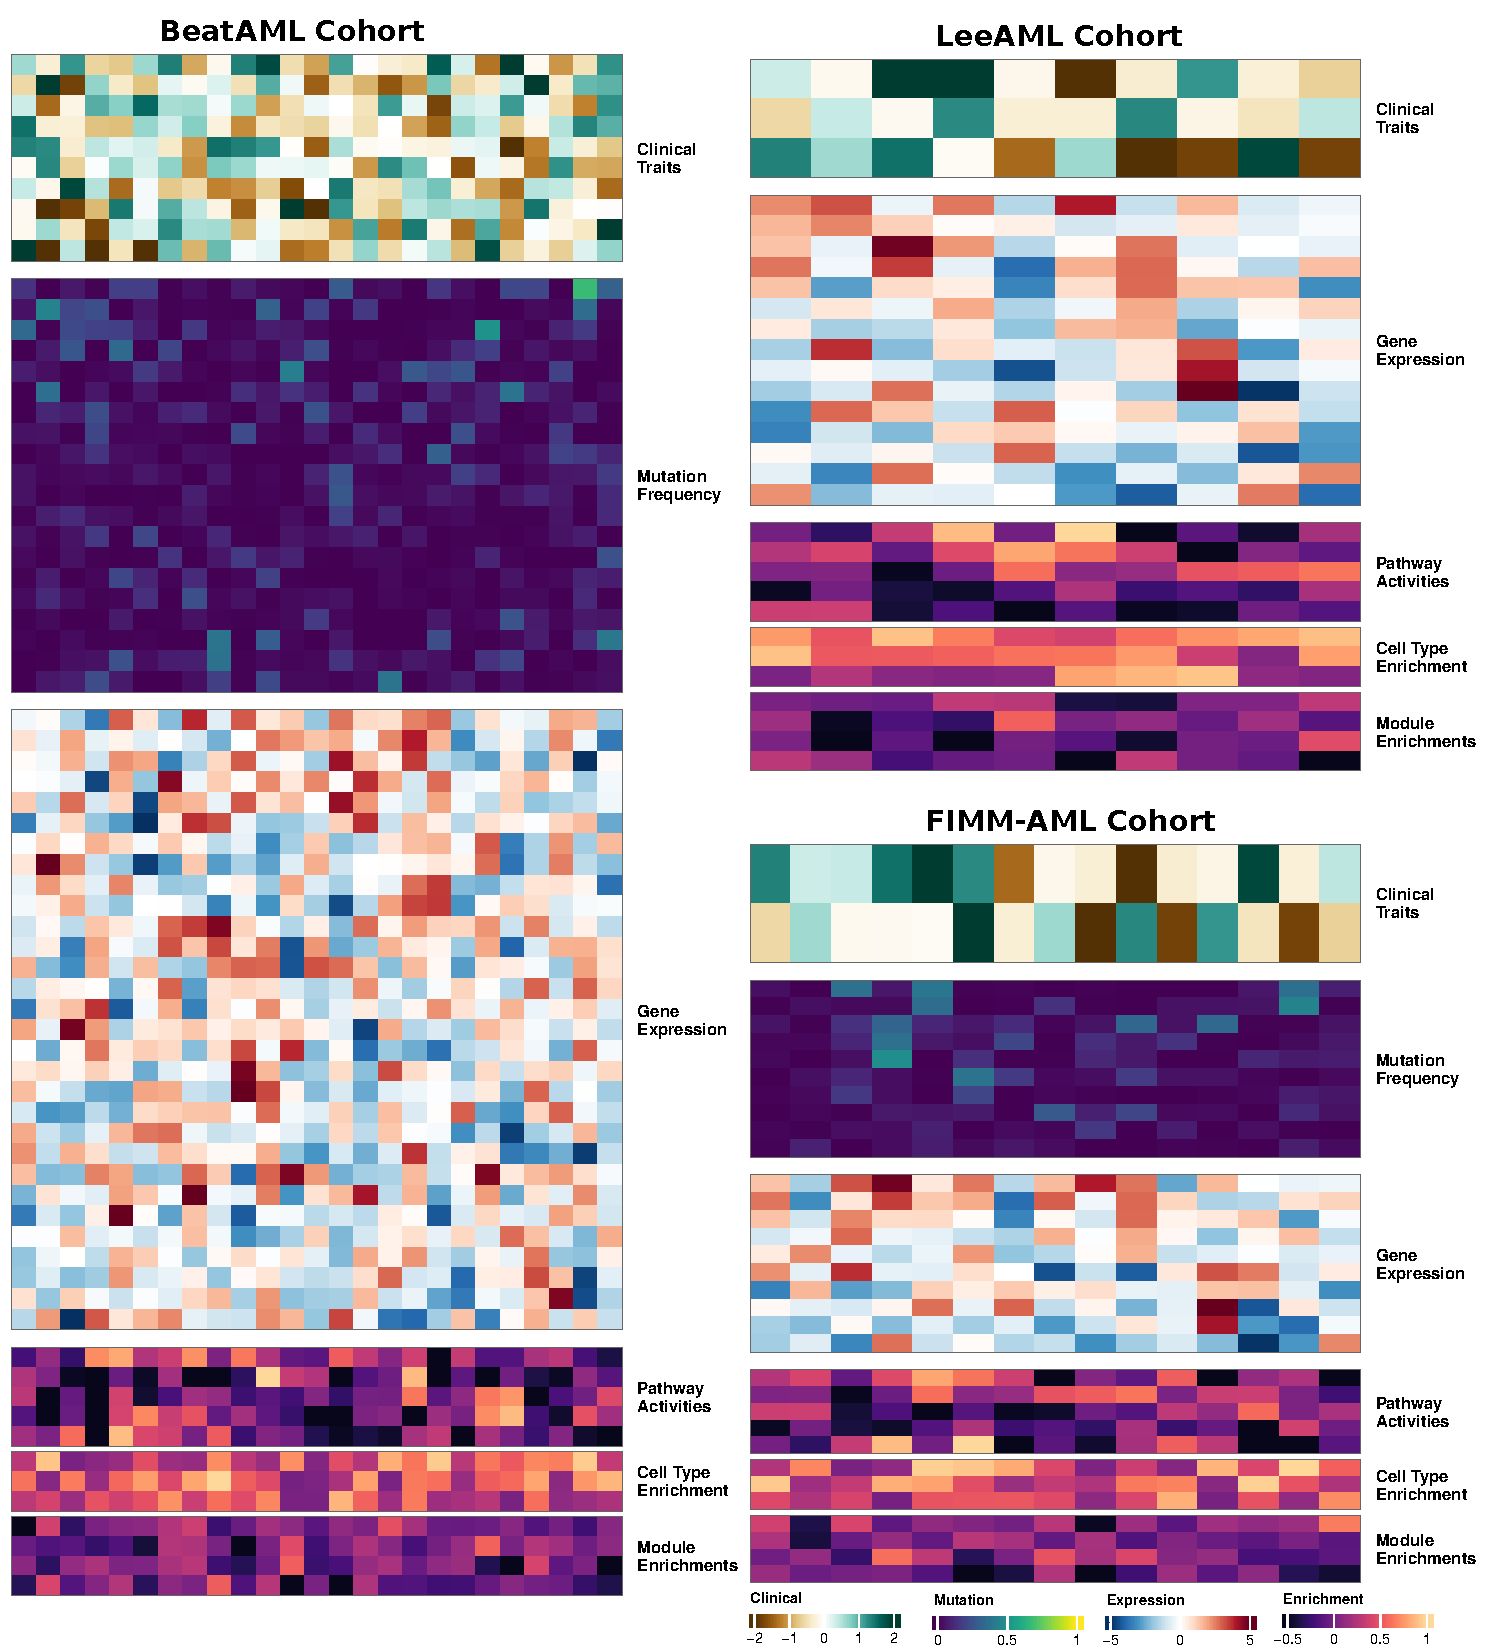
\includegraphics[width=0.96\textwidth]{figures/MultiOmics_Rep.pdf}
    \caption{Multi-omics landscape of acute myeloid leukemia (AML) across three independent cohorts (BeatAML, LeeAML and FIMM-AML). Rows correspond to clinical, genomic, transcriptomic, functional features; columns correspond to patient samples.}
    \label{fig:fig1}
\end{figure}

\textbf{Mutated Genes and Types}: Somatic variant calls from DNA-Seq were incorporated to evaluate mutation frequencies and types as available in the original BeatAML cohort \cite{bottomly2022integrative}. %The frequency of mutation in the top mutated genes and corresponding mutation types served as additional features. 
Figure~\ref{fig:fig1} highlights these representative patient characteristics across BeatAML, LeeAML and FIMM-AML cohorts as a heatmap respectively.

%%%%%%%%%%%%%%%%%%%%%%%%%%%%%%%%%%%
\subsection{Drug Data and Multi-Modal Fingerprint Generation}\label{sec2.5}
We collected drug response data from the BeatAML dataset. A total of $165$ unique drugs were available, of which $150$ were represented in the training set (Waves~1+2) and $153$ in the held-out test set (Waves~3+4); $15$ drugs appeared exclusively in the test set, enabling assessment of generalization to unseen compounds. After intersecting with available drug feature representations, $150$ test drugs were included in the final evaluation. We derived four complementary molecular representations for each drug:

\begin{enumerate}
    \item \textbf{Physico-Chemical Feature Representation (PC):} Drug molecular features were derived using RDKit \cite{bento2020open}: $148$ non-redundant and non-correlated molecular descriptors, $30$ graph-theoretic features computed via NetworkX (v3.5), Morgan circular fingerprints (radius~3, 128~bits), and MACCS structural keys (167~bits, first bit inactive). This 473-dimensional representation was recently identified as optimal for predicting diverse molecular properties \cite{harod2025effichem}; the full feature list is provided in Supplementary Table S1.

    \item \textbf{Knowledge-Distilled Embeddings (KD-Embed):} Fixed-length Knowledge Distilled (KD) latent vectors were produced by a Teacher Forcing Long Short-Term Memory (TF-LSTM) sequence-to-sequence autoencoder \cite{mall2021modeling} trained on $\approx\!2.5$ million compounds from PubChem \cite{kim2025pubchem} and the MOSES benchmark \cite{10.3389/fphar.2020.565644} (see Figure \ref{fig:fig_lstm}. Overall, $96.7\%$ of reconstructed compounds were valid as determined by RDKit, with mean categorical cross-entropy of $0.001$.
    
    \item \textbf{ChemBERTa Embeddings:} We encoded drug SMILES strings using ChemBERTa \cite{chithrananda2020chemberta}, a transformer pre-trained on 77~million compounds from PubChem using masked language modeling, producing $384$-dimensional contextual representations that capture chemical substructure and neighbourhood information. Embeddings were extracted zero-shot, without fine-tuning the ChemBERTa model.
    \item \textbf{MolFormer Embeddings:} We generated $768$-dimensional embeddings using MolFormer \cite{ross2022large}, a large-scale rotary-position transformer pre-trained on $\sim\!1.1$ billion SMILES strings from PubChem and ZINC. MolFormer designed to capture long-range molecular dependencies and global structural properties. As with ChemBERTa, embeddings were extracted in zero-shot fashion.
\end{enumerate}

Figure~\ref{fig:fig2} illustrates the TF-LSTM based drug embedding pipeline and the drug-pathway distance estimation scheme.

\begin{figure}[!ht]
    \centering
    \begin{subfigure}{0.99\linewidth}
        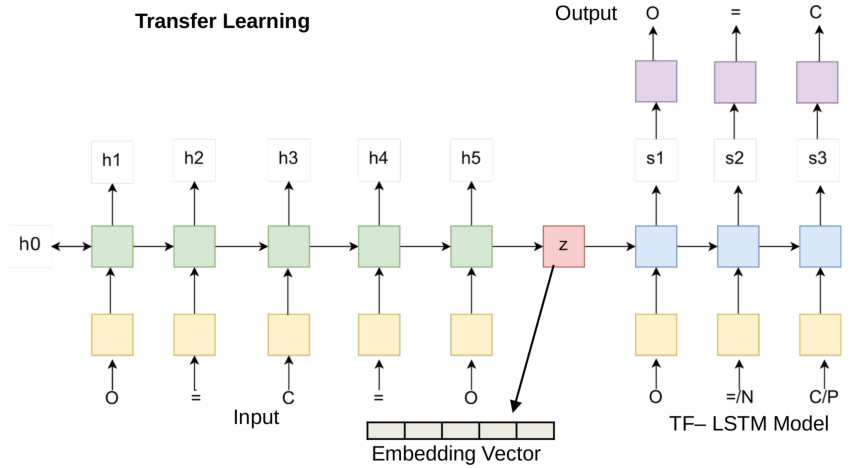
\includegraphics[width=0.9\textwidth]{figures/TFLSTM.pdf}
        \caption{TF-LSTM model \cite{mall2021modeling} generating KD-Embed vectors for compounds.}
        \label{fig:fig_lstm}
    \end{subfigure}
    \begin{subfigure}{0.99\textwidth}
        \centering
        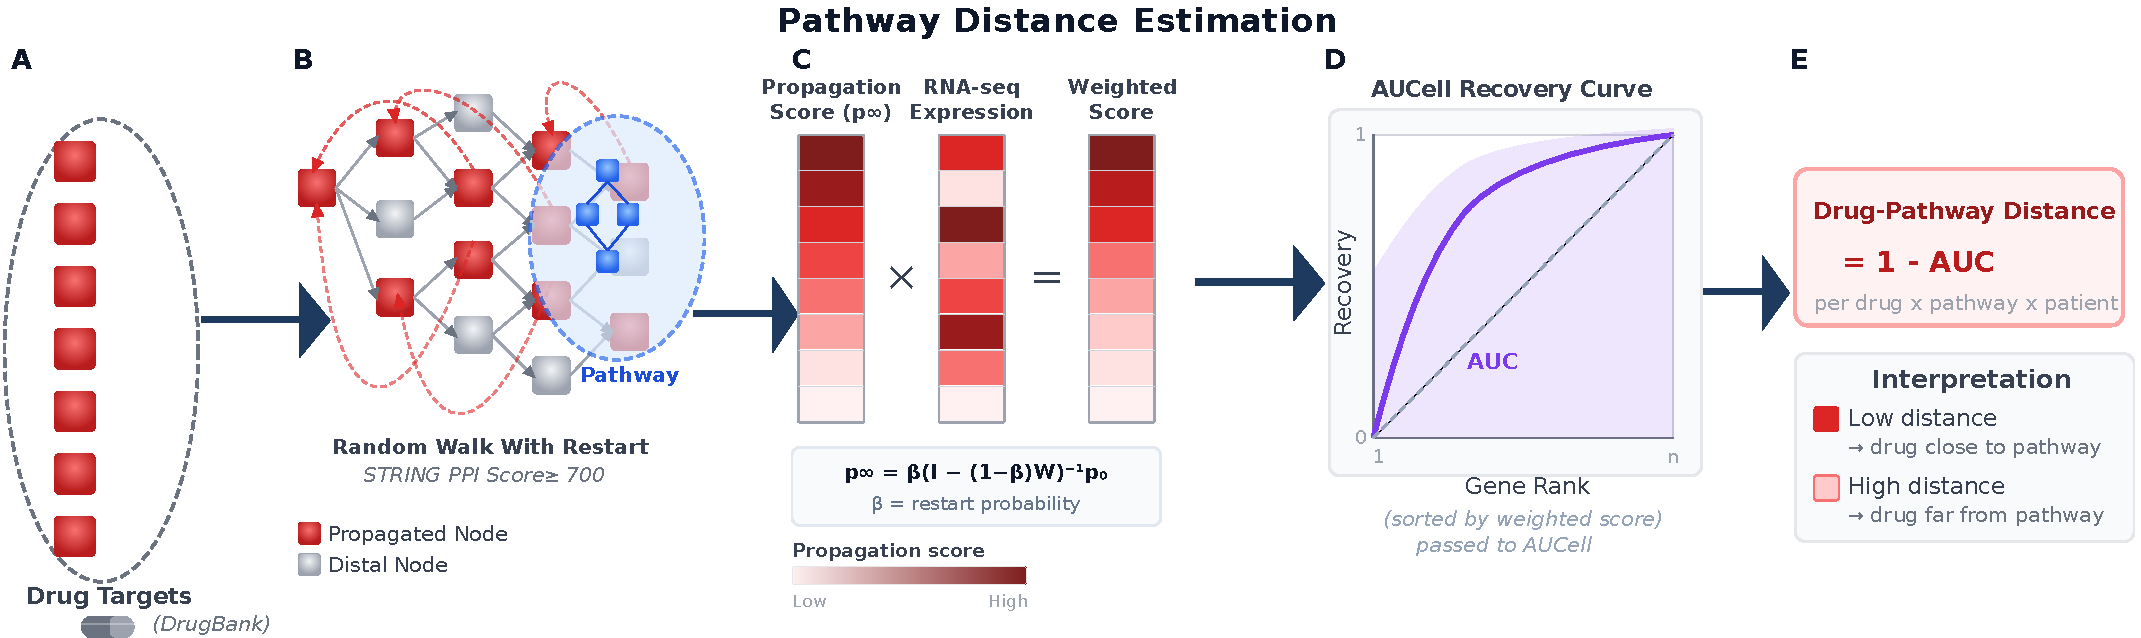
\includegraphics[width=0.99\textwidth]{figures/DrugPathwayDistance.pdf}
        \caption{Steps involved in patient-specific drug-pathway distance estimation via random-walk propagation and AUCell scoring.}
        \label{fig:fig_drugpathway_auc}
    \end{subfigure}
    \caption{Drug embedding generation and drug--pathway distance calculation.}
    \label{fig:fig2}
\end{figure}

%%%%%%%%%%%%%%%%%%%%%%%%%%%%%%%%%%%
\subsection{Drug Pathway Distance Estimation}\label{sec2.6}
To estimate a computational proximity of each drug to individual oncogenic pathways in a patient-specific manner, we exploit drug target information available from DrugBank \cite{knox2024drugbank}. Drug targets (genes/proteins) serve as starting points in the human protein-protein interaction (PPI) network obtained from the STRING database, retaining only interactions with strong experimental evidence (score $\ge 700$).

Starting from drug targets, network propagation via a random-walk with restart (RWR) approach \cite{sherif2022immune,mall2013kernel} produces a propagation vector representing the global proximity of each protein to a given drug. To obtain a patient-specific local propagation vector, we weight each protein's propagation score by the corresponding gene expression from RNA-seq. The resulting vector reflects how ``close'' an oncogenic pathway is to a given drug in the molecular context of a specific patient: if pathway member genes rank highly in the sorted propagation vector, the drug has close proximity to that pathway, and vice versa. Pathway proximity was estimated using the AUCell package (v1.24.0) \cite{aibar2017scenic}, computing the AUC, where higher AUC corresponds to lower distance i.e. closer drug-pathway proximity for a given patient (see Fig \ref{fig:fig_drugpathway_auc}).

%%%%%%%%%%%%%%%%%%%%%%%%%%%%%%%%%%%%%%%%%%
\subsection{Training and Test Data Preparation}\label{sec2.7}
Using the approach described above, we assembled comprehensive patient representations comprising: mutation profiles (frequency and type for top mutated genes), gene expression profiles (150 most variable genes and oncogenes), and enrichment scores (pathway activity, module enrichment, cell state). Drug representations were one of the four molecular encodings (PC, KD-Embed, ChemBERTa, MolFormer) supplemented by drug target annotations from DrugBank \cite{knox2024drugbank} and patient-specific drug-pathway AUC proximity scores.

The merged BeatAML training and held-out test datasets were constructed by performing inner joins between the drug response table, patient feature table (keyed by patient ID), and drug feature table (keyed by compound ID) using the \texttt{merge} function in \texttt{pandas}. The resulting training set contains $33{,}803$ patient-drug records and the test set contains $18{,}826$ records. Feature dimensionality ranges from $277$ to $2,034$ depending on the drug representation used and the feature group ablation configuration. An analogous pipeline was applied to LeeAML and FIMM-AML, generating merged drug-patient feature matrices for external evaluation. The overall PREDICT-AML workflow is illustrated in Figure~\ref{fig:fig3}.

\begin{figure}[!ht]
    \centering
    
\includegraphics[width=0.95\textwidth]{jtrm_images/Figure3.pdf}
    \caption{The PREDICT-AML framework: from multi-omics BeatAML data collection and feature engineering through model training, cross-validation, and external validation on independent LeeAML and FIMM-AML cohorts.}
    \label{fig:fig3}
\end{figure}

%%%%%%%%%%%%%%%%%%%%%%%%%%%%%%%%%%%
\subsection{Machine Learning Models}\label{sec2.8}
We developed and trained diverse machine learning models to predict drug response using combined molecular, genomic, and clinical features together with drug representations.

\textbf{Standard models} included generalized linear regression (GLR) \cite{nelder1972generalized}, support vector regression (SVR) \cite{chandorkar2015fixed}, Random Forests (RF) \cite{breiman2001random}, XGBoost \cite{chen2016xgboost}, LightGBM \cite{ke2017lightgbm} and CatBoost \cite{prokhorenkova2018catboost}. \textbf{Deep learning models} processing the SMILES string directly included convolutional neural networks (CNN) \cite{sermanet2012convolutional}, LSTM \cite{gers2000learning}, graph attention networks (GAT) \cite{velivckovic2017graph}, and graph convolutional networks (GCN) \cite{kipf2017semi}.

\textbf{TabPFN} \cite{hollmann2023tabpfn} serves as the primary model in PREDICT-AML. TabPFN (Tabular Prior-data Fitted Networks) is a transformer-based model that treats tabular datasets as contexts and generates predictions in a single forward pass without gradient-based optimization at inference time. It is pre-trained via meta-learning on a large collection of synthetic datasets sampled from a structured Bayesian prior, allowing it to perform in-context learning and naturally handle the heterogeneous, high-dimensional, mixed-type feature matrices characteristic of multi-omics drug response data. Hyperparameters for all tree-based and TabPFN models were optimized using Optuna \cite{akiba2019optuna} with 5-fold cross-validation on the BeatAML training set.

Performance metrics included mean absolute error (MAE), root mean squared error (RMSE), Pearson correlation ($r_{pc}$), Spearman correlation ($r_{sc}$), and coefficient of determination (R$^2$). Lower MAE and RMSE and higher $r_{pc}$, $r_{sc}$, and R$^2$ indicate better performance.

%%%%%%%%%%%%%%%%%%%%%%%%%%%%%%%%%%%
\subsection{Cross-Validation Strategies}\label{sec2.9}
To rigorously assess different aspects of model generalizability, we evaluated TabPFN under three distinct 5-fold cross-validation (CV) strategies on the BeatAML training set:

\begin{enumerate}
    \item \textbf{Random CV:} Patient-drug pairs are assigned randomly to folds. This standard strategy tests interpolation within the observed distribution of patients and drugs.
    \item \textbf{Patient-stratified CV (PS-CV):} Folds are partitioned by patient identity, ensuring no patient appears in both training and validation. This evaluates the model's ability to predict drug response for new, previously unseen patients - the most clinically relevant scenario.
    \item \textbf{Drug-stratified CV (DS-CV):} Folds are partitioned by drug identity, ensuring no drug appears in both training and validation. This evaluates generalization to structurally or mechanistically novel drugs not encountered during training.
\end{enumerate}

Each configuration is independently evaluated with all four drug molecular representations (PC, KD-Embed, ChemBERTa, MolFormer), yielding 12 experimental conditions for any machine learning technique including the primary TabPFN analysis.

%%%%%%%%%%%%%%%%%%%%%%%%%%%%%%%%%%%%%%%%%%%%%
\section{Results}\label{sec3}

\subsection{Benchmarking Machine Learning Models on BeatAML}\label{sec3.1}
We benchmarked the full suite of classical machine learning and deep learning models on the BeatAML training (Waves 1+2) and test (Waves 3+4) sets. Figure~\ref{fig:fig4}A shows the distribution of the area under the drug response curve (AUC) between training (Y\_train) and test (Y\_test) sets. AUC values range between 0 and 300, with no statistically significant distributional difference between sets ($p > 0.05$, Wilcoxon rank-sum test \cite{mann1947test}). A heatmap of normalized predicted drug responses across all patient samples and inhibitors is provided in Supplementary Fig.~2, illustrating the heterogeneity of predicted sensitivity across the BeatAML cohort.

\begin{figure}[!ht]
    \centering
    
\includegraphics[width=0.92\textwidth]{jtrm_images/Figure4.pdf}
    \caption{Performance comparison of machine learning models for predicting drug response of AML patients on the BeatAML cohort. Panels show: (A) AUC distribution between training and test sets; (B--K) scatter plots of predicted vs.\ observed AUC for the best-performing instance of each model class on the test set; (L) top-10 patient profiles and top-10 drugs for which CatBoost predictions are most accurate; (M) bottom-10 patient profiles and bottom-10 drugs with lowest predictive accuracy.}
    \label{fig:fig4}
\end{figure}

\begin{table}[!ht]
\centering
\caption{\textbf{Best-performing configuration per model on BeatAML (Waves~1+2 training, Waves~3+4 test).}
One row per model; drug representation selected by highest held-out test $r_{pc}$ with smallest generalization gap.
PS-CV = 5-fold patient-stratified cross-validation (the clinically meaningful benchmark; mean\,$\pm$\,std across folds).
$\%\Delta r_{pc} = (r_{\text{PS-CV}} - r_{\text{Test}})/r_{\text{PS-CV}} \times 100$; smaller = better generalization;
negative values (GAT+FFNN rows) indicate test $r_{pc}$ marginally exceeds PS-CV mean.
\textbf{Bold} = PREDICT-AML (TabPFN) with the ablation-optimal feature configuration
(all patient feature groups + KD-Embed; see Supplementary Table~S3 for full ablation; Supplementary Table~S2 for all model--drug representation combinations).}
\label{table:benchmark_compact}
%\resizebox{\textwidth}{!}{
\footnotesize{
\begin{tabular}{lllccccr}
\toprule
\textbf{Model} & \textbf{Class} & \textbf{Drug Rep.} &
\textbf{PS-CV MAE} & \textbf{Test MAE} &
\textbf{PS-CV $r_{pc}$} & \textbf{Test $r_{pc}$} & $\%\Delta r_{pc}$ \\
\midrule
\textbf{TabPFN} & \textbf{Transformer} & \textbf{KD-Embed} &
$\mathbf{31.054 \pm 0.742}$ & $\mathbf{37.712}$ & $\mathbf{0.724 \pm 0.015}$ & $\mathbf{0.690}$ & $\mathbf{4.7}$ \\
LightGBM & Tree ensemble & PC & $32.099 \pm 1.953$ & $38.399$ & $0.718 \pm 0.031$ & $0.681$ & $5.2$ \\
CatBoost & Tree ensemble & KD-Embed & $32.478 \pm 0.527$ & $38.391$ & $0.699 \pm 0.020$ & $0.676$ & $3.3$ \\
XGBoost & Tree ensemble & ChemBERTa & $32.804 \pm 1.834$ & $38.918$ & $0.704 \pm 0.018$ & $0.673$ & $4.4$ \\
LSTM & DL (SMILES) & MolFormer & $31.859 \pm 0.552$ & $39.532$ & $0.717 \pm 0.010$ & $0.652$ & $9.1$ \\
RF & Tree ensemble & ChemBERTa & $33.831 \pm 0.917$ & $40.076$ & $0.676 \pm 0.026$ & $0.651$ & $3.7$ \\
CNN & DL (SMILES) & MolFormer & $32.106 \pm 0.498$ & $40.520$ & $0.711 \pm 0.010$ & $0.651$ & $8.4$ \\
GCN+FFNN & DL (graph) & MolFormer & $32.547 \pm 0.567$ & $39.936$ & $0.696 \pm 0.010$ & $0.647$ & $7.0$ \\
GAT+FFNN & DL (graph) & MolFormer & $35.158 \pm 0.803$ & $40.403$ & $0.695 \pm 0.008$ & $0.633$ & $8.9$ \\
GLR & Linear & MolFormer & $35.391 \pm 1.238$ & $41.412$ & $0.660 \pm 0.015$ & $0.619$ & $6.2$ \\
LSSVR & Linear & MolFormer & $35.632 \pm 1.174$ & $42.220$ & $0.655 \pm 0.013$ & $0.601$ & $8.2$ \\
\bottomrule
\end{tabular}
}
\end{table}

Table~\ref{table:benchmark_compact} summarises the best-performing drug representation for each of the 11 benchmark models, selected by held-out test $r_{pc}$ on Waves~3+4; full results for all drug representations are provided in Supplementary Table~S2. PREDICT-AML (TabPFN with KD-Embed, ablation-optimised feature set) achieves the highest test $r_{pc} = 0.690$ and lowest Test MAE $= 37.712$, with a generalization gap of $\%\Delta r_{pc} = 4.7\%$. Among classical models, tree-based gradient-boosted ensembles (LightGBM, CatBoost, XGBoost, RF) consistently outperform linear and neural-network alternatives. The best tree-based model, LightGBM (PC), achieves test $r_{pc} = 0.681$ and MAE $= 38.399$; CatBoost (KD-Embed) achieves test $r_{pc} = 0.676$ and MAE $= 38.391$. Deep learning models processing SMILES or molecular graphs directly (CNN, LSTM, GAT+FFNN, GCN+FFNN) achieve test $r_{pc} = 0.633$--$0.652$ (PS-CV $r_{pc} = 0.695$--$0.717$) and MAE $= 39.5$--$40.5$ under their best molecular representations (MolFormer in all cases). Linear models (GLR, LSSVR) achieve test $r_{pc} = 0.601$--$0.619$, reflecting limited capacity to capture non-linear feature interactions. An advantage of tree-based models is interpretability via feature importance \cite{mall2018rgbm,louppe2013understanding}; SHAP-based interpretability for the best CatBoost model is provided in Supplementary Figs.~6--7. SHAP-based interpretability for the best PREDICT-AML (TabPFN, KD-Embed) configuration on the held-out test set is presented in Section~\ref{sec3.7}.

%%%%%%%%%%%%%%%%%%%%%%%%%%%%%%%%%%%
\subsection{Patient-Stratified Evaluation as the Clinically Meaningful Benchmark}\label{sec3.2}
A central finding of this study is that the choice of cross-validation (CV) strategy has a decisive impact on the apparent predictive performance of drug response models, and that standard random CV substantially overestimates a model's real-world utility. To quantify this effect, we evaluated TabPFN across all four drug molecular representations under three CV strategies: patient-stratified CV (PS-CV), drug-stratified CV (DS-CV), and random CV. Numerical results are provided in Table~\ref{table:tabpfn_cv}, and an overview across all metrics and drug representations is shown in Figure~\ref{fig:fig_tabpfn}.

\begin{figure}[!ht]
    \centering
    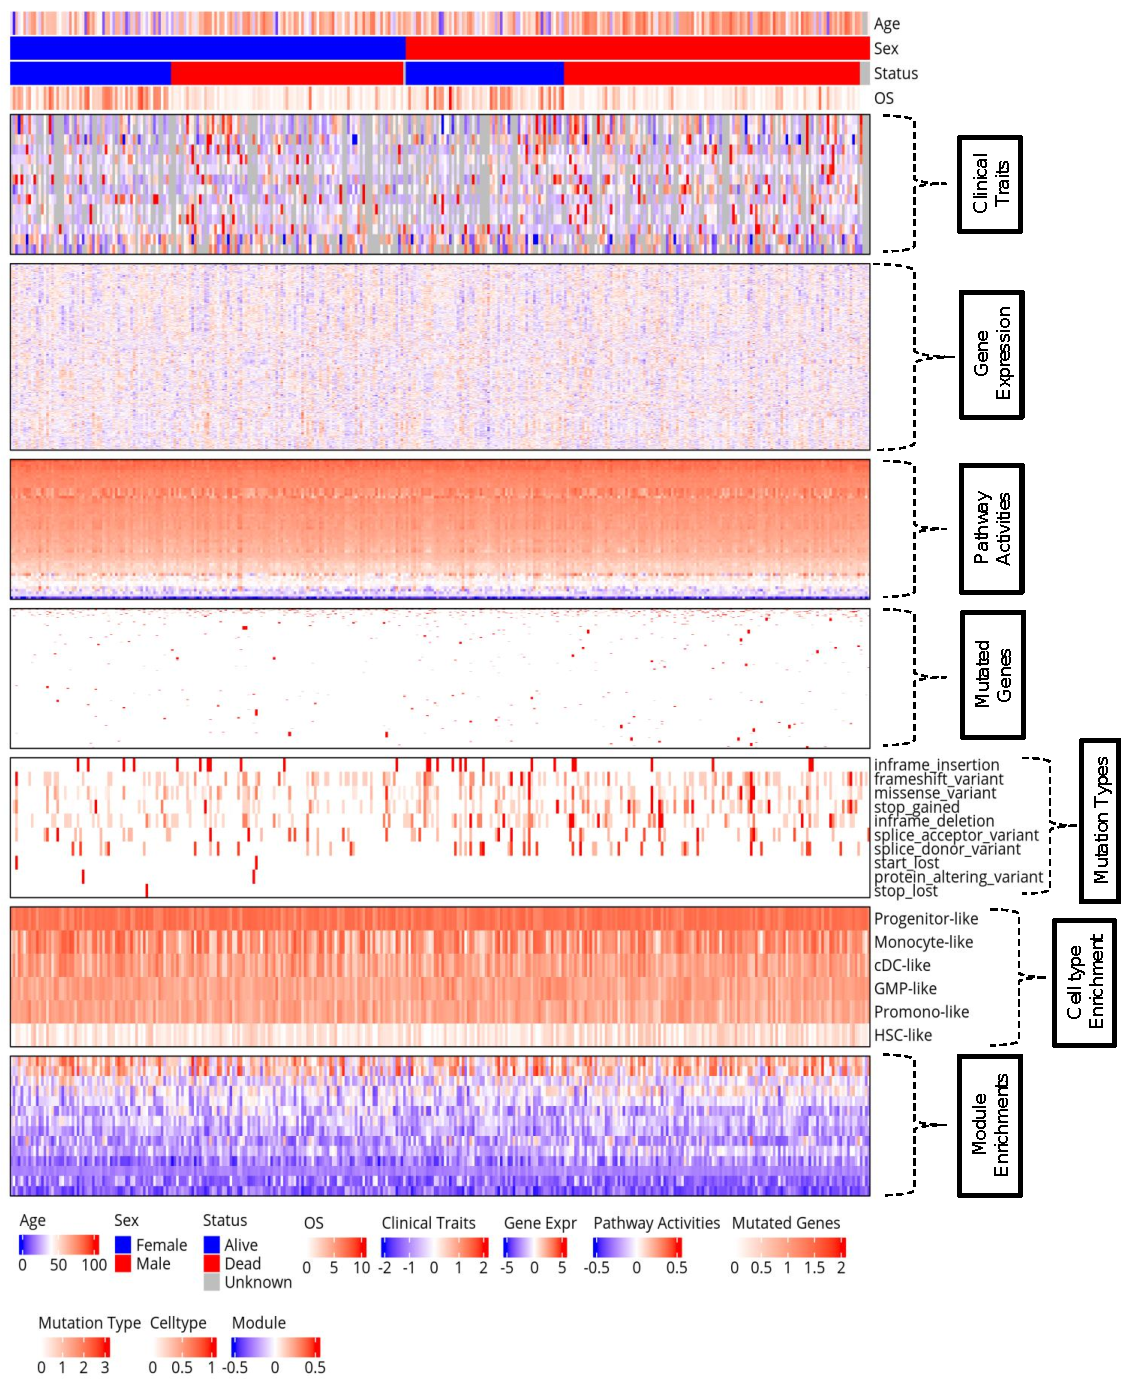
\includegraphics[width=0.97\textwidth]{figures/Figure1.pdf}
    \caption{TabPFN cross-validation performance on BeatAML under three CV strategies (patient-stratified, drug-stratified, random) and four drug molecular representations (Only\_PC, SMILES-LS, ChemBERTa, MolFormer). Panels display MAE, RMSE, R$^2$, Pearson $r_{pc}$, and Spearman $r_{sc}$. Patient-stratified CV (PS-CV) reflects the clinically relevant scenario of predicting response for new patients; random CV consistently inflates all performance metrics relative to PS-CV.}
    \label{fig:fig_tabpfn}
\end{figure}

\begin{table}[!ht]
\centering
\caption{Cross-validation performance of TabPFN on BeatAML under three strategies and four drug molecular representations. \textbf{Bold} indicates the best patient-stratified (PS-CV) result---the clinically meaningful benchmark. $^\dagger$Random CV rows inflate apparent performance due to patient--drug pair leakage across folds; see text. DS-CV = drug-stratified CV.}
\label{table:tabpfn_cv}
%\resizebox{0.99\textwidth}{!}{
\footnotesize{
\begin{tabular}{|l|l|c|c|c|c|c|}
\hline
\textbf{Drug Repr.} & \textbf{CV Strategy} & \textbf{MAE} & \textbf{RMSE} & \textbf{R$^2$} & $r_{pc}$ & $r_{sc}$ \\
\hline
PC & PS-CV & $31.790 \pm 1.451$ & $43.513 \pm 2.963$ & $0.508 \pm 0.029$ & $0.712 \pm 0.021$ & $0.706 \pm 0.012$ \\
PC & DS-CV & $46.743 \pm 4.247$ & $58.955 \pm 5.269$ & $0.096 \pm 0.028$ & $0.306 \pm 0.045$ & $0.268 \pm 0.042$ \\
PC & Random$^\dagger$ & $26.290 \pm 0.285$ & $36.710 \pm 0.295$ & $0.645 \pm 0.002$ & $0.803 \pm 0.001$ & $0.796 \pm 0.003$ \\
\hline
KD Embed & \textbf{PS-CV} & $\mathbf{31.453 \pm 0.959}$ & $43.181 \pm 1.526$ & $0.512 \pm 0.019$ & $\mathbf{0.716 \pm 0.013}$ & $\mathbf{0.711 \pm 0.013}$ \\
KD Embed & DS-CV & $45.841 \pm 4.645$ & $58.740 \pm 6.166$ & $0.121 \pm 0.054$ & $0.337 \pm 0.082$ & $0.311 \pm 0.078$ \\
KD Embed & Random$^\dagger$ & $26.047 \pm 0.288$ & $36.444 \pm 0.272$ & $0.651 \pm 0.002$ & $0.807 \pm 0.002$ & $0.799 \pm 0.003$ \\
\hline
ChemBERTa & PS-CV & $31.574 \pm 1.417$ & $43.230 \pm 1.860$ & $0.512 \pm 0.032$ & $0.715 \pm 0.022$ & $0.709 \pm 0.028$ \\
ChemBERTa & DS-CV & $45.285 \pm 3.859$ & $57.409 \pm 4.639$ & $0.150 \pm 0.065$ & $0.377 \pm 0.088$ & $0.348 \pm 0.096$ \\
ChemBERTa & Random$^\dagger$ & $26.009 \pm 0.266$ & $36.423 \pm 0.249$ & $0.651 \pm 0.003$ & $0.807 \pm 0.002$ & $0.800 \pm 0.003$ \\
\hline
MolFormer & \textbf{PS-CV} &  $31.592 \pm 1.327$ & $\mathbf{43.138 \pm 2.793}$ & $\mathbf{0.513 \pm 0.034}$ & ${0.716 \pm 0.024}$ & ${0.708 \pm 0.019}$ \\
MolFormer & DS-CV & $45.227 \pm 1.978$ & $57.499 \pm 3.396$ & $0.139 \pm 0.019$ & $0.372 \pm 0.024$ & $0.346 \pm 0.030$ \\
MolFormer & Random$^\dagger$ & $25.995 \pm 0.259$ & $36.373 \pm 0.219$ & $0.652 \pm 0.003$ & $0.808 \pm 0.001$ & $0.800 \pm 0.003$ \\
\hline
\end{tabular}
}
\end{table}

\textbf{Patient-stratified CV is the primary benchmark.} In PS-CV, each fold withholds an entire subset of patients from training, directly simulating the clinical scenario in which a model must generalize to new individuals not seen during development. Under PS-CV, all four drug representations achieve consistent performance: $r_{pc} \approx 0.712$--$0.716$ (MAE $\approx 31.5$--$31.8$). The top-performing configuration is MolFormer ($r_{pc} = 0.716 \pm 0.024$, MAE $= 31.592 \pm 1.327$; SMILES-LS performs comparably at $r_{pc} = 0.716 \pm 0.013$), demonstrating that the model captures transferable patient-level transcriptomic and genomic signals.

\textbf{Random CV overestimates generalization.} A critical observation from Table~\ref{table:tabpfn_cv} is that random CV yields $r_{pc} \approx 0.803$--$0.808$ (MAE $\approx 26.0$--$26.3$) for all drug representations---a Pearson correlation approximately $13\%$ higher than the PS-CV estimate. This inflation arises because random fold assignment places different drug--patient pairs from the same patients in both training and validation, allowing the model to implicitly interpolate between known patient states rather than extrapolating to genuinely new individuals. The $\sim\!22\%$ lower MAE under random CV (26.0 vs.\ 31.6) similarly overstates predictive accuracy. These results underscore that random CV is an inappropriate benchmark for clinical deployment, where predictions are always made for patients the model has not encountered before. Full random CV benchmark results for all 11 models across all drug representations are provided in Supplementary Table~S5.

\textbf{Drug-stratified CV reveals chemical generalization limits.} Under DS-CV, performance drops substantially to $r_{pc} \approx 0.306$--$0.377$ (MAE $\approx 45.2$--$46.7$), reflecting the inherent difficulty of predicting response to structurally novel drugs. Here, chemical language models provide a clear advantage: ChemBERTa ($r_{pc} = 0.377 \pm 0.088$) and MolFormer ($r_{pc} = 0.372 \pm 0.024$) outperform physicochemical-only representations ($r_{pc} = 0.306 \pm 0.045$), demonstrating that pre-training on large molecular databases encodes transferable structural knowledge. This advantage does not manifest under PS-CV or random CV---where patient features dominate---confirming that drug representation quality is the primary bottleneck specifically for novel-compound generalization. Full DS-CV benchmark results for all 11 models across all drug representations are provided in Supplementary Table~S4.

Scatter plots of predicted versus observed AUC values for the best-performing TabPFN configuration (MolFormer) across CV strategies are shown in Figure~\ref{fig:tabpfn_scatter}.

\begin{figure}[!ht]
    \centering
    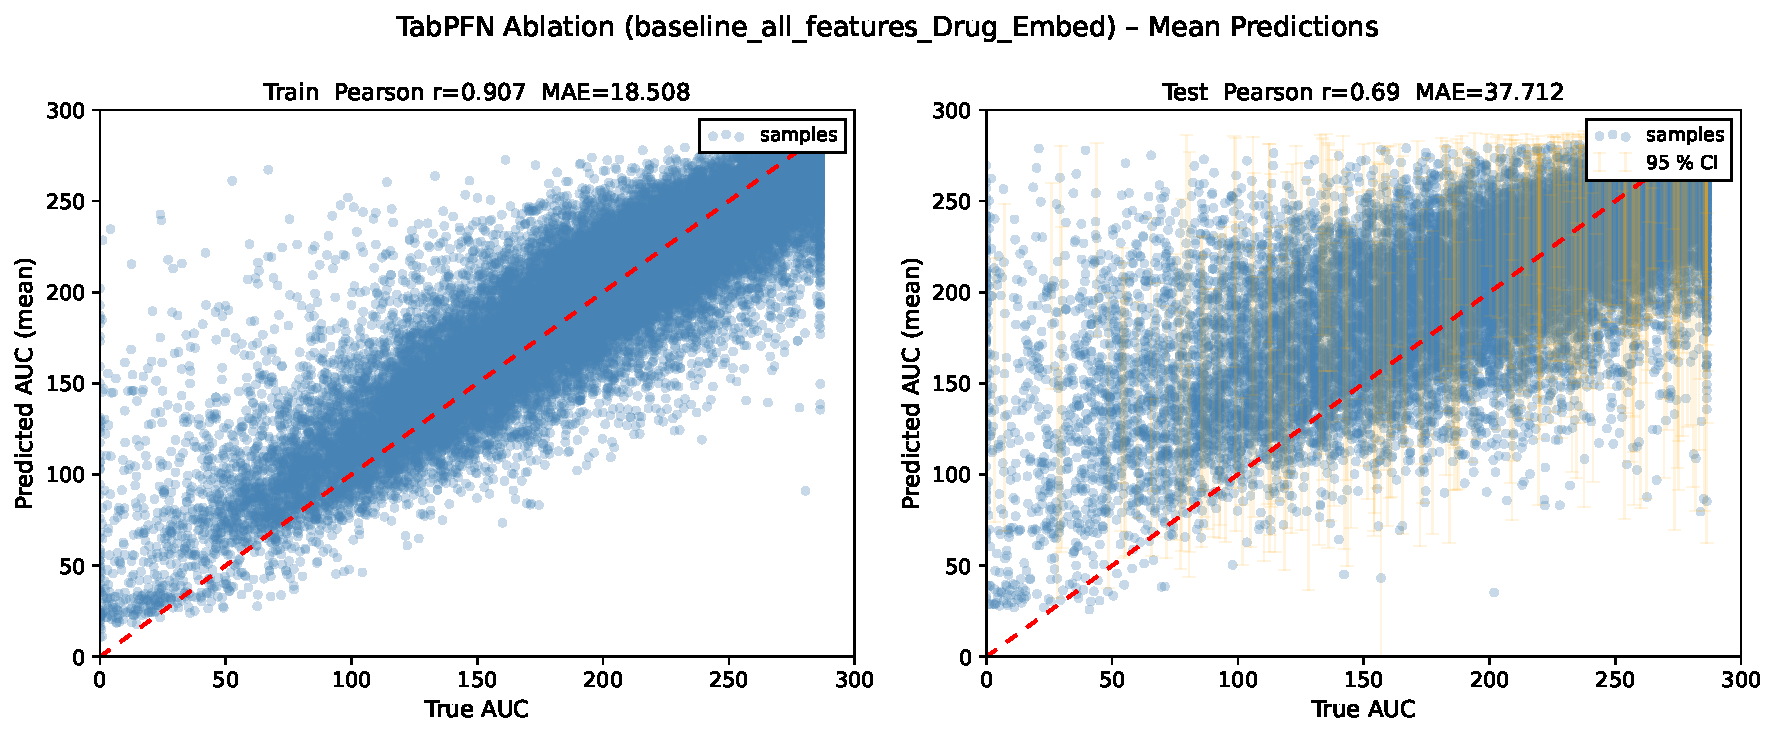
\includegraphics[width=0.95\textwidth]{figures/TabPFN_predictions_scatter.pdf}
    \caption{Predicted versus observed AUC values for the best-performing TabPFN configuration (MolFormer drug embeddings) on BeatAML. Each point represents a patient--drug pair; the diagonal line indicates perfect prediction. The patient-stratified CV (PS-CV) result ($r_{pc} = 0.716$) is the clinically meaningful evaluation; random CV ($r_{pc} = 0.808$) inflates apparent performance by excluding the patient-level generalization challenge from validation.}
    \label{fig:tabpfn_scatter}
\end{figure}

%%%%%%%%%%%%%%%%%%%%%%%%%%%%%%%%%%%
\subsection{Ablation Study on Feature Group Contributions}\label{sec3.3}
We performed a systematic ablation study on BeatAML to quantify the contribution of individual feature groups to TabPFN prediction performance. Feature groups were: (i)~Gene Expression (150 most variable genes + oncogenes); (ii)~Mutation profiles; (iii)~Pathway enrichment scores; (iv)~Cell state and module enrichment (Clinical, CellType, Module). These were evaluated individually and in pairwise and triple combinations with each of the three drug representations (Only\_PC, SMILES-LS, MolFormer+PC). Baseline models using all features (all four groups combined) served as references.

Representative ablation prediction scatter plots are shown in Supplementary Fig.~3 for the baseline configurations (PC and KD-Embed drug representations). Under random CV, baseline models using all features with Only\_PC drugs ($r_{pc} = 0.803 \pm 0.002$, MAE $= 26.381 \pm 0.247$), SMILES-LS drugs ($r_{pc} = 0.806 \pm 0.001$), and combined PC+Embed drugs ($r_{pc} = 0.807 \pm 0.001$) all perform comparably, with marginal gains from richer drug representations. Under drug-stratified CV, baseline models achieve $r_{pc} \approx 0.312$--$0.342$ (MAE $\approx 46.2$--$45.8$), and single-group models using only gene expression or clinical/cell-type/module features achieve similar drug-stratified $r_{pc} \approx 0.314$--$0.338$, confirming that drug representation quality---not patient feature complexity---is the primary bottleneck for novel-drug generalization.

The full ablation results (all feature group combinations and all CV strategies) are provided in Supplementary Table~S3 and Supplementary Fig.~3.

%%%%%%%%%%%%%%%%%%%%%%%%%%%%%%%%%%%
\subsection{External Validation on LeeAML}\label{sec3.4}
To assess transferability beyond the BeatAML cohort, we applied the trained PREDICT-AML model to the independent LeeAML dataset \cite{lee2018machine}. The LeeAML cohort uses the same AUC drug sensitivity metric as BeatAML, enabling direct comparison of predicted and measured drug responses. We evaluated all four drug representation configurations (Only\_PC, SMILES-LS, ChemBERTa, MolFormer) on the 49 drugs common to both datasets. Figure~\ref{fig:leeaml} shows the predicted versus observed AUC scatter plots for all configurations.

\begin{figure}[!ht]
    \centering
    
\includegraphics[width=0.97\textwidth]{figures/LeeAML_all_configs_scatter.pdf}
    \caption{External validation of PREDICT-AML on the LeeAML cohort \cite{lee2018machine}. Each panel shows predicted versus observed AUC values for one of the four drug molecular representations (Only\_PC, SMILES-LS, ChemBERTa, MolFormer) on the 49 drugs common between BeatAML and LeeAML. The diagonal line indicates perfect agreement.}
    \label{fig:leeaml}
\end{figure}

The external validation confirms that PREDICT-AML generalizes to an independent AML cohort with distinct patient demographics, treatment protocols, and sample processing workflows. The SMILES-LS (Embed) representation achieves the most consistent performance on the LeeAML patient-stratified evaluation (Supplementary Fig.~4 shows the best-performing single-configuration result for KD Embed). ChemBERTa and MolFormer representations also demonstrate meaningful correlation, with variability reflecting the smaller cohort size ($n = 30$) and the differing distribution of drug response values between institutions.

%%%%%%%%%%%%%%%%%%%%%%%%%%%%%%%%%%%
\subsection{External Validation on FIMM-AML}\label{sec3.5}
We further validated PREDICT-AML on the FIMM-AML cohort \cite{malani2022implementing}, which uses DSS as its drug sensitivity metric and covers a substantially broader pharmacological space (540 drugs). The 78 drugs overlapping with BeatAML were used for evaluation.

Figure~\ref{fig:fimmaml} shows the predicted versus observed scatter plots for all four drug representation configurations on FIMM-AML.

\begin{figure}[!ht]
    \centering
    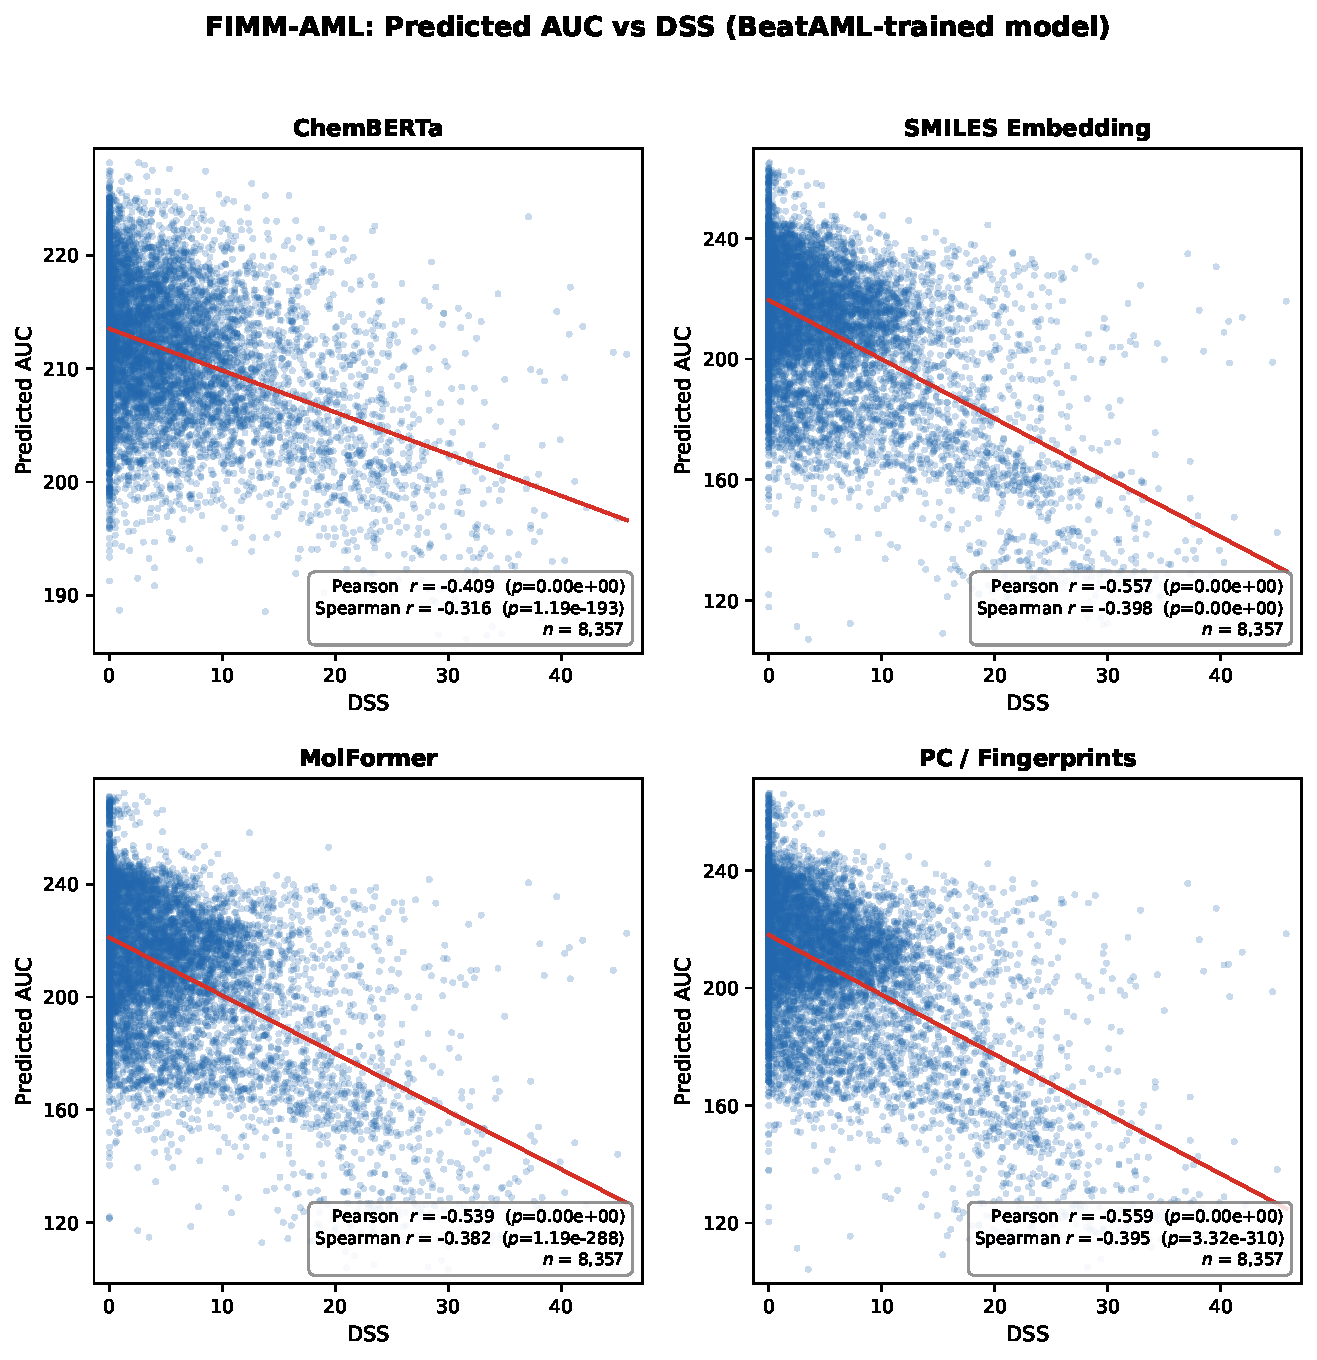
\includegraphics[width=0.97\textwidth]{figures/FIMMAML_all_configs_scatter.pdf}
    \caption{External validation of PREDICT-AML on the FIMM-AML cohort \cite{malani2022implementing}. Each panel shows predicted AUC (BeatAML scale) versus observed DSS values for one drug representation configuration on the 78 drugs common between BeatAML and FIMM-AML. Color encodes drug identity; the diagonal trend indicates cross-platform predictive agreement.}
    \label{fig:fimmaml}
\end{figure}

The cross-platform setting---predicting AUC-scale values that are compared against DSS measurements---is inherently more challenging than the LeeAML evaluation, given the systematic differences in drug response quantification methodology between FIMM and BeatAML. Despite this, the model demonstrates meaningful rank correlations between predicted and observed drug sensitivity values across FIMM-AML patients, validating that the transcriptomic and genomic signals captured by PREDICT-AML are informative across distinct clinical institutions and drug sensitivity platforms. The best-performing configuration (KD Embed) scatter plot comparing predicted AUC against DSS scores is provided in Supplementary Fig.~4.

%%%%%%%%%%%%%%%%%%%%%%%%%%%%%%%%%%%
\subsection{Prediction Confidence Interval Analysis}\label{sec3.6}
A key advantage of the TabPFN framework is its ability to provide calibrated prediction uncertainty estimates alongside point predictions. For the best-performing BeatAML configuration (MolFormer, random CV), we computed $95\%$ confidence intervals (CIs) for each patient--drug pair in the test set using an ensemble of TabPFN predictors. Figure~\ref{fig:ci} presents the distribution of CI widths across all test predictions.

\begin{figure}[!ht]
    \centering
    
\includegraphics[width=0.75\textwidth]{figures/CI_width_distribution.pdf}
    \caption{Distribution of $95\%$ prediction confidence interval (CI) widths for the best TabPFN configuration (MolFormer, random CV) on the BeatAML test set. Narrower CIs indicate higher prediction certainty; the distribution reveals that the majority of patient--drug predictions carry well-characterized uncertainty, with a subset of highly uncertain predictions corresponding to drugs tested on fewer patient samples.}
    \label{fig:ci}
\end{figure}

The CI width distribution (Figure~\ref{fig:ci}) reveals that the majority of patient--drug pair predictions carry moderate uncertainty (median CI width $\approx 100$--$120$ AUC units), while a long right tail corresponds to predictions with higher uncertainty---typically for drugs tested on fewer patient samples. This uncertainty quantification provides a clinically actionable signal: predictions with narrow CIs can be relied upon with greater confidence when informing therapeutic selection, whereas those with wide CIs flag cases where additional experimental evidence may be warranted before acting on the model output.

%%%%%%%%%%%%%%%%%%%%%%%%%%%%%%%%%%%
\subsection{SHAP-based Interpretability of PREDICT-AML}\label{sec3.7}
To understand which features drive individual predictions of the best PREDICT-AML configuration (TabPFN with KD-Embed, full feature set), we computed SHAP (SHapley Additive exPlanations) values \cite{lundberg2017unified} for all patient--drug pairs in the held-out test set. The base value---the model's average prediction across the test cohort---is $\approx 197.3$ AUC units, and each SHAP value additively explains a prediction's deviation from this baseline.

Figure~\ref{fig:shap_global} shows the global feature importance for the test set as a bar chart of mean $|\text{SHAP}|$ values alongside a beeswarm summary plot.

\begin{figure}[!ht]
    \centering
    \begin{subfigure}[b]{0.47\textwidth}
        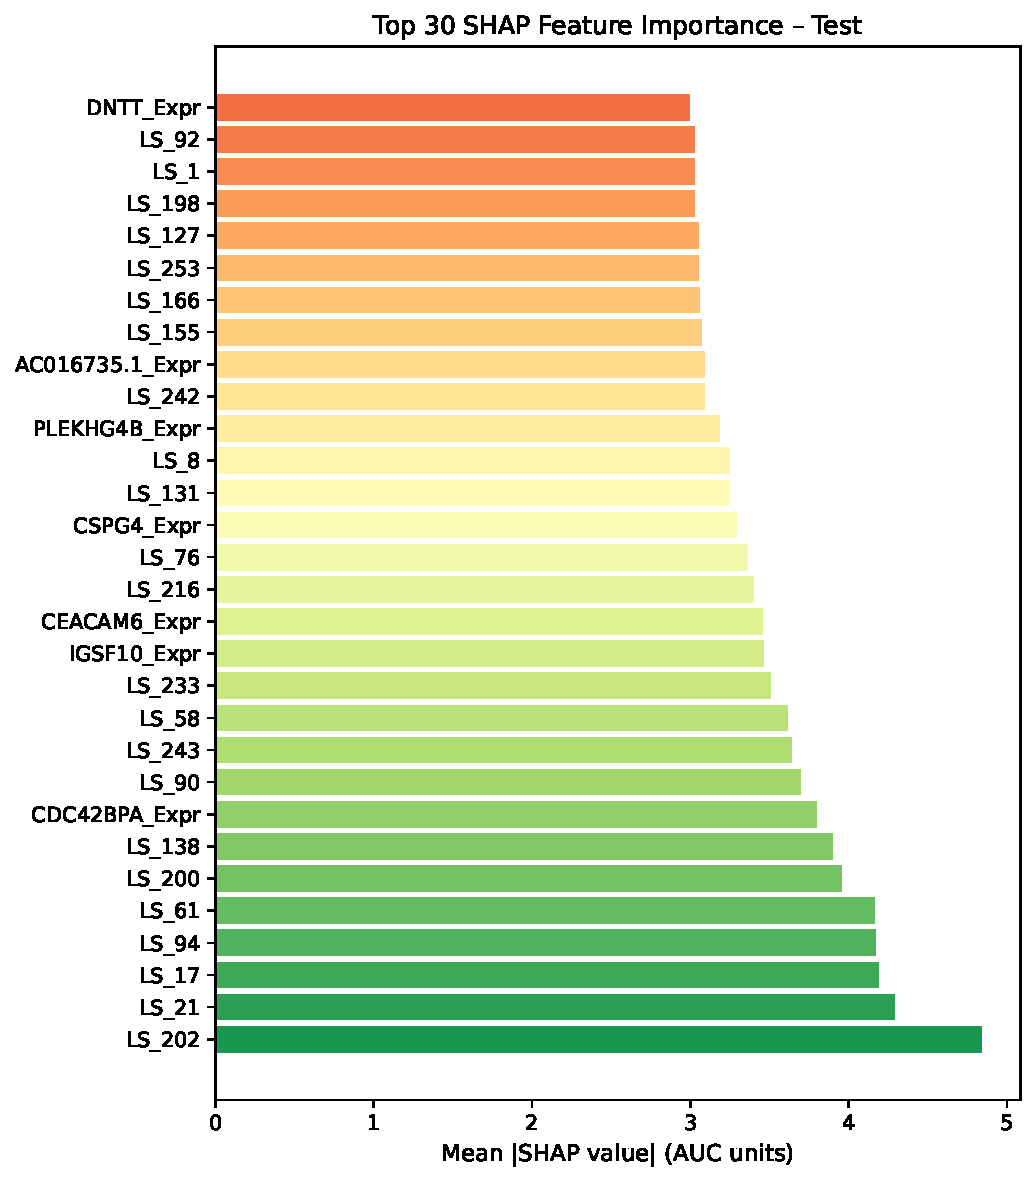
\includegraphics[width=\textwidth]{figures/SHAP_importance_bar_test.pdf}
        \caption{Mean $|\text{SHAP}|$ bar chart (top 20 features)}
        \label{fig:shap_bar}
    \end{subfigure}
    \hfill
    \begin{subfigure}[b]{0.50\textwidth}
        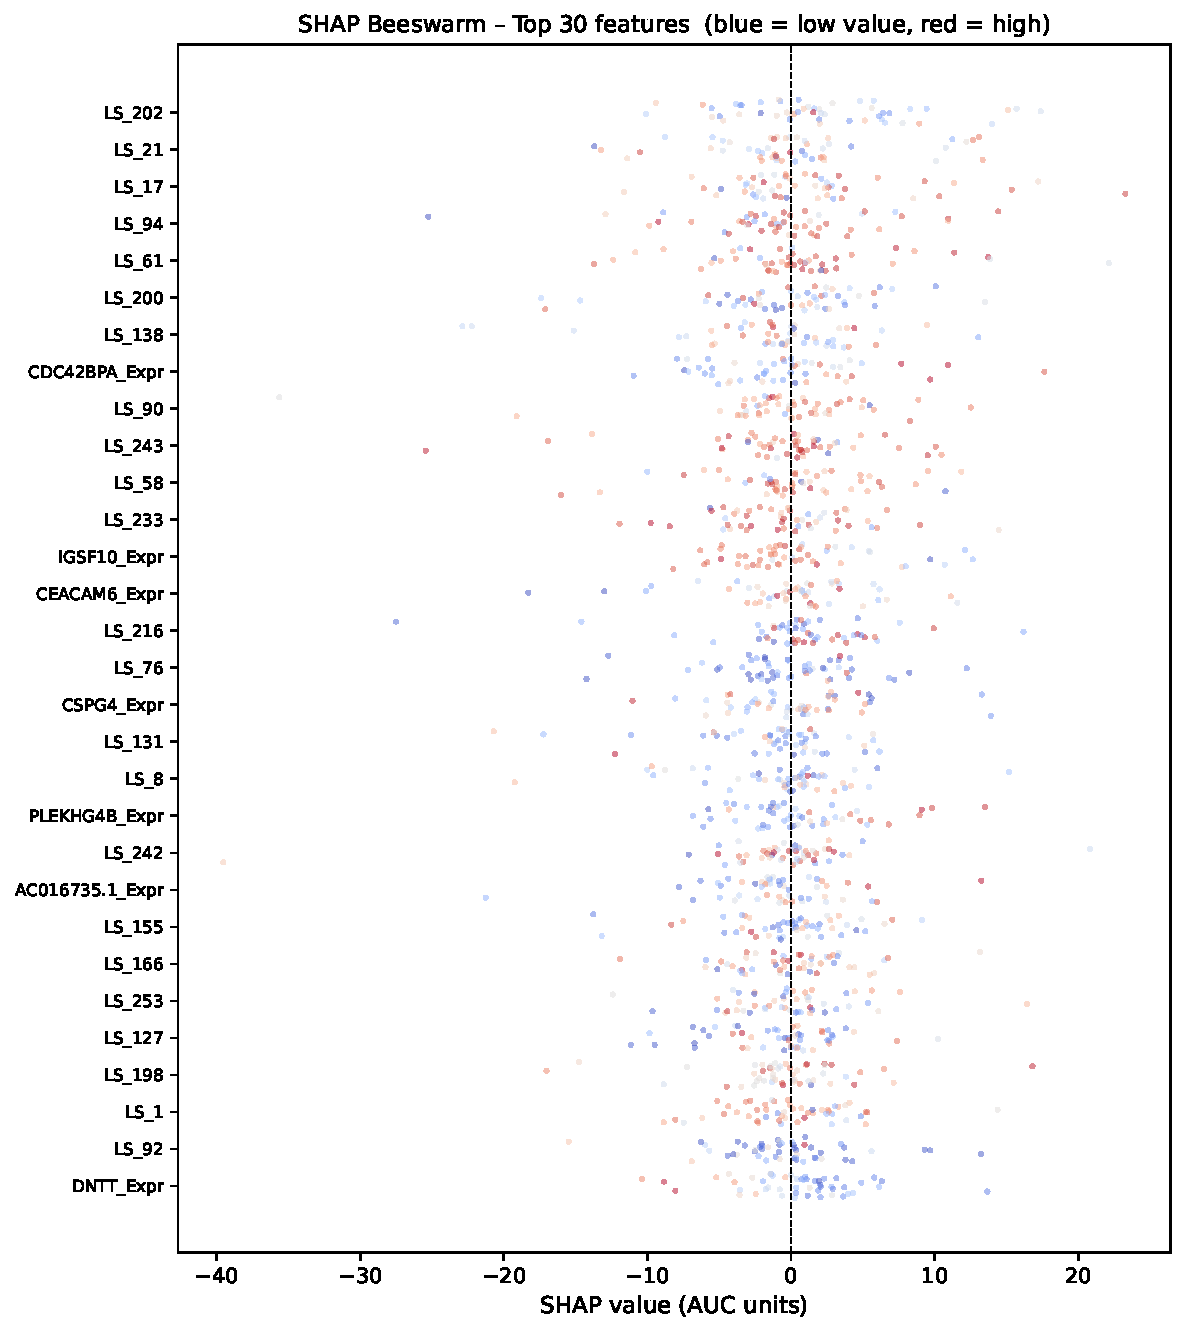
\includegraphics[width=\textwidth]{figures/SHAP_beeswarm_test.pdf}
        \caption{Beeswarm summary plot}
        \label{fig:shap_beeswarm}
    \end{subfigure}
    \caption{Global SHAP feature importance for PREDICT-AML on the held-out BeatAML test set (TabPFN, KD-Embed configuration). (A)~Mean absolute SHAP values for the top 20 features. Drug embedding dimensions (LS\_*) dominate the ranking, with patient gene expression features (e.g., \textit{CDC42BPA}, \textit{IGSF10}, \textit{CEACAM6}, \textit{CSPG4}) appearing among the leading patient-level predictors. (B)~Beeswarm plot showing the distribution of SHAP values across all test patient--drug pairs for each feature; colour encodes the feature value (red $=$ high, blue $=$ low). Wide beeswarm spreads reflect features with heterogeneous influence across the cohort.}
    \label{fig:shap_global}
\end{figure}

Drug embedding dimensions from the KD-Embed representation (LS\_202, LS\_21, LS\_17, LS\_94, LS\_61, LS\_200, LS\_138) collectively dominate the global importance ranking, confirming that chemical properties of the drug are the primary determinants of the predicted AUC response. This is expected in a multi-drug prediction framework where drug identity must account for the bulk of variance in response. Among patient-level features, the gene expression of \textit{CDC42BPA} (CDC42 binding protein kinase $\alpha$; mean $|\text{SHAP}| \approx 3.80$), \textit{IGSF10} ($\approx 3.46$), \textit{CEACAM6} ($\approx 3.46$), and \textit{CSPG4} ($\approx 3.29$) stand out as the leading transcriptomic predictors, indicating that the model captures biologically meaningful patient-specific signals modulating drug sensitivity.

To illustrate how SHAP values explain individual predictions, Figure~\ref{fig:shap_individual} presents waterfall plots for two representative test-set samples: a correctly predicted sensitive patient--drug pair and a correctly predicted resistant pair.

\begin{figure}[!ht]
    \centering
    \begin{subfigure}[b]{0.48\textwidth}
        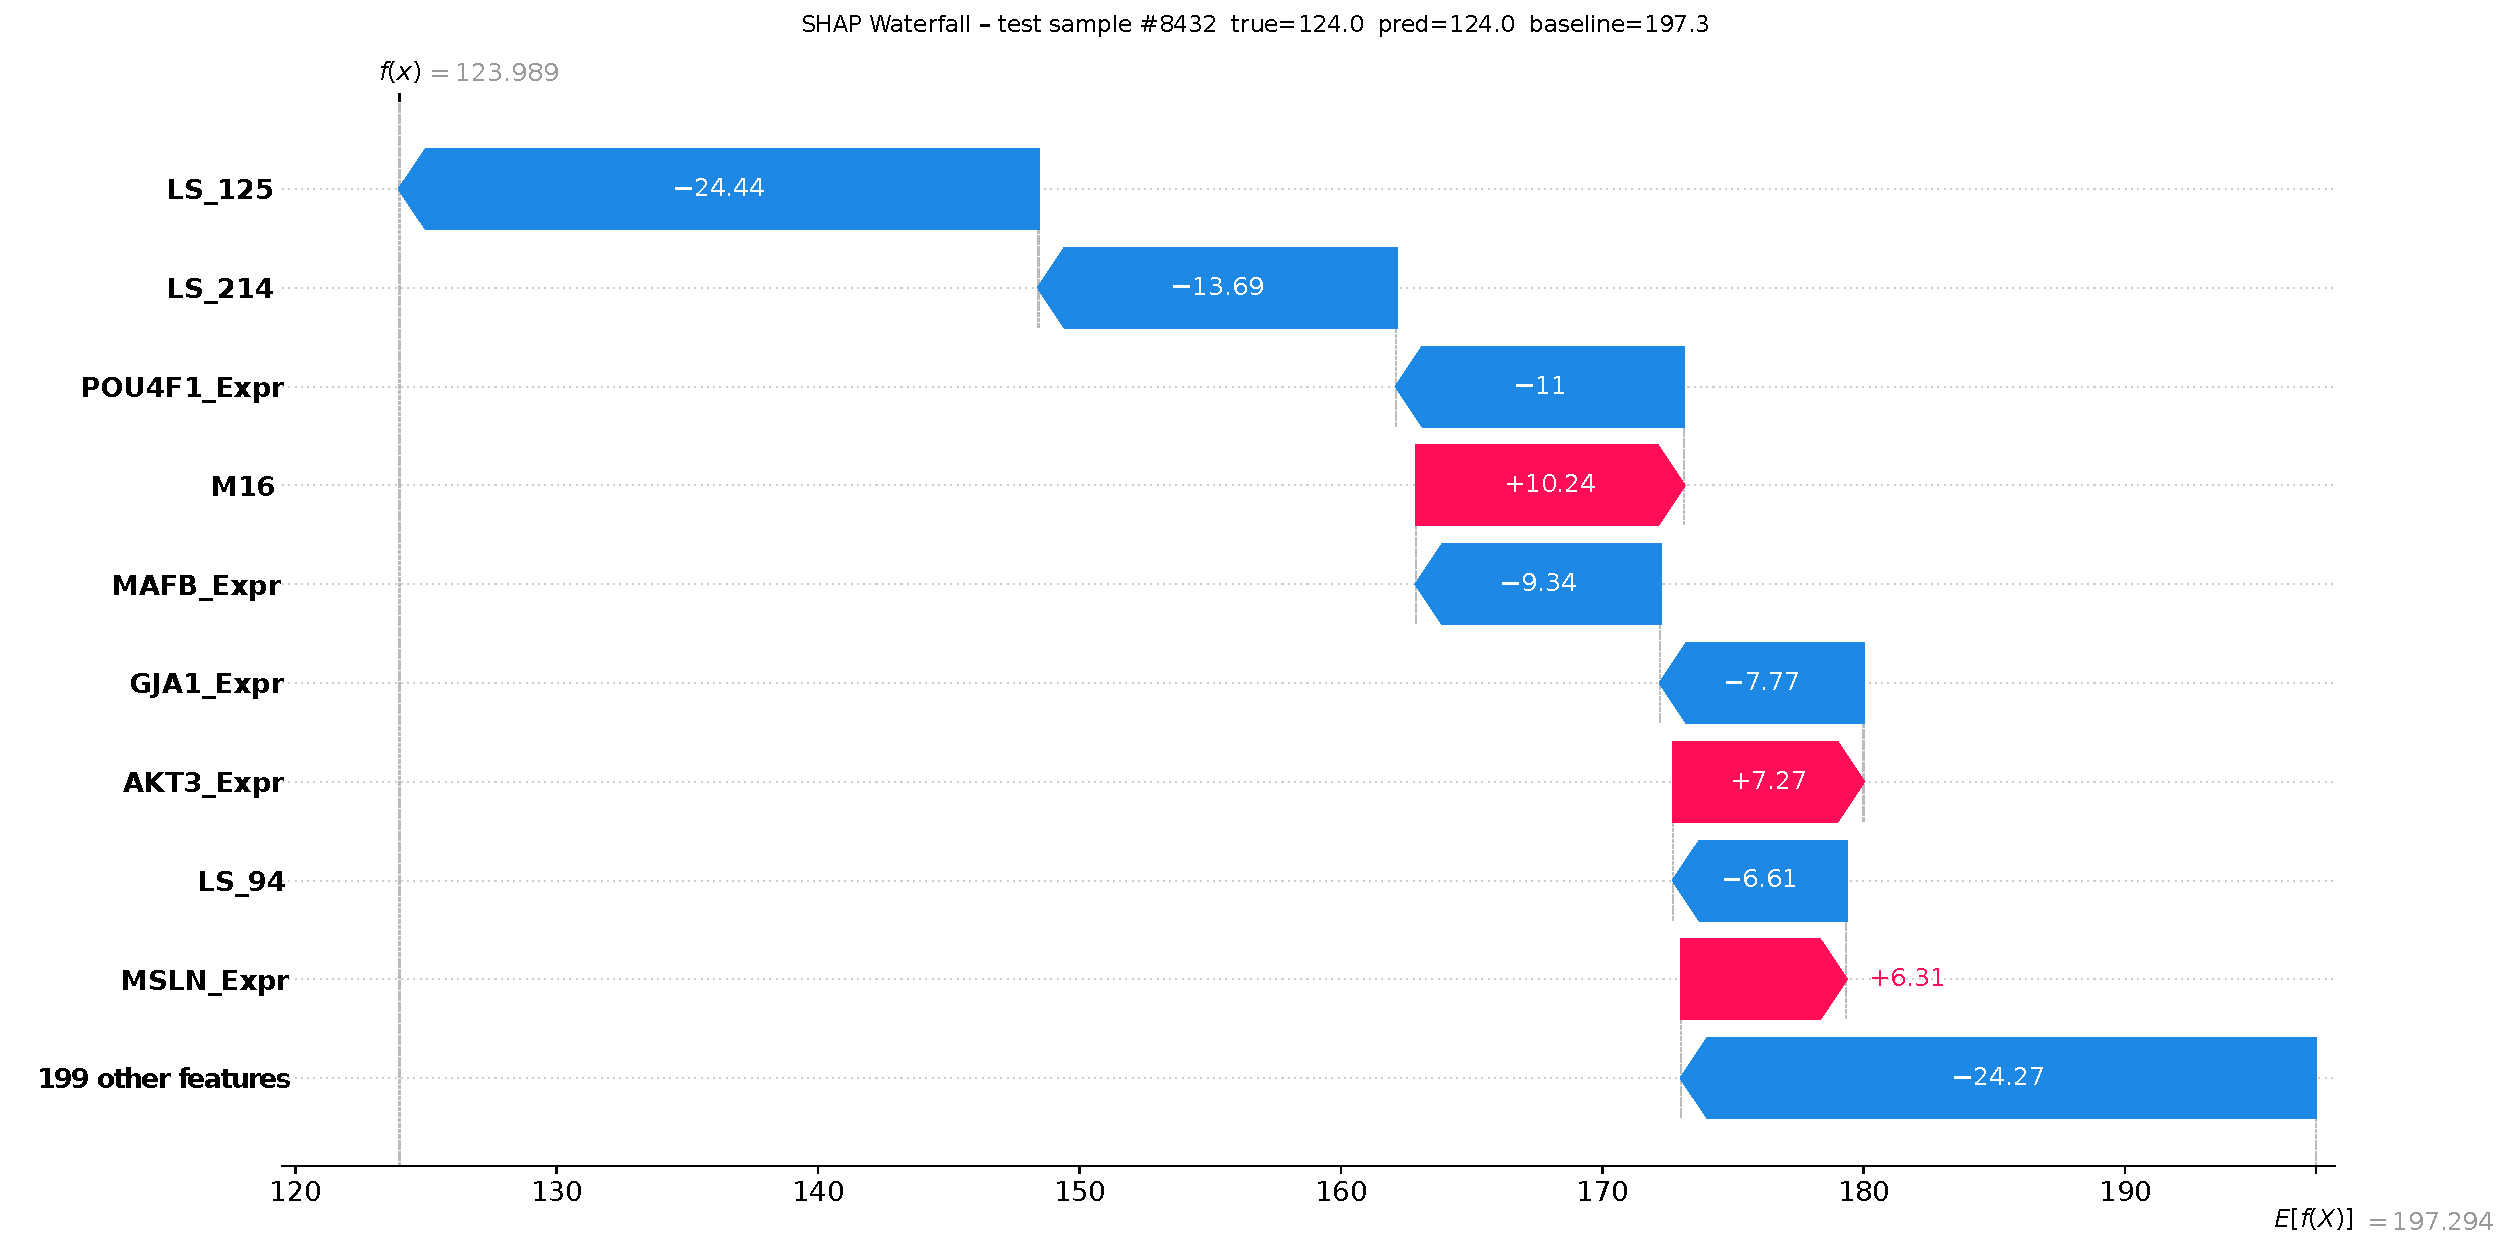
\includegraphics[width=\textwidth]{figures/SHAP_sensitivity_idx8432.pdf}
        \caption{Sensitive: true AUC $= 124.0$, predicted $= 124.0$}
        \label{fig:shap_sens}
    \end{subfigure}
    \hfill
    \begin{subfigure}[b]{0.48\textwidth}
        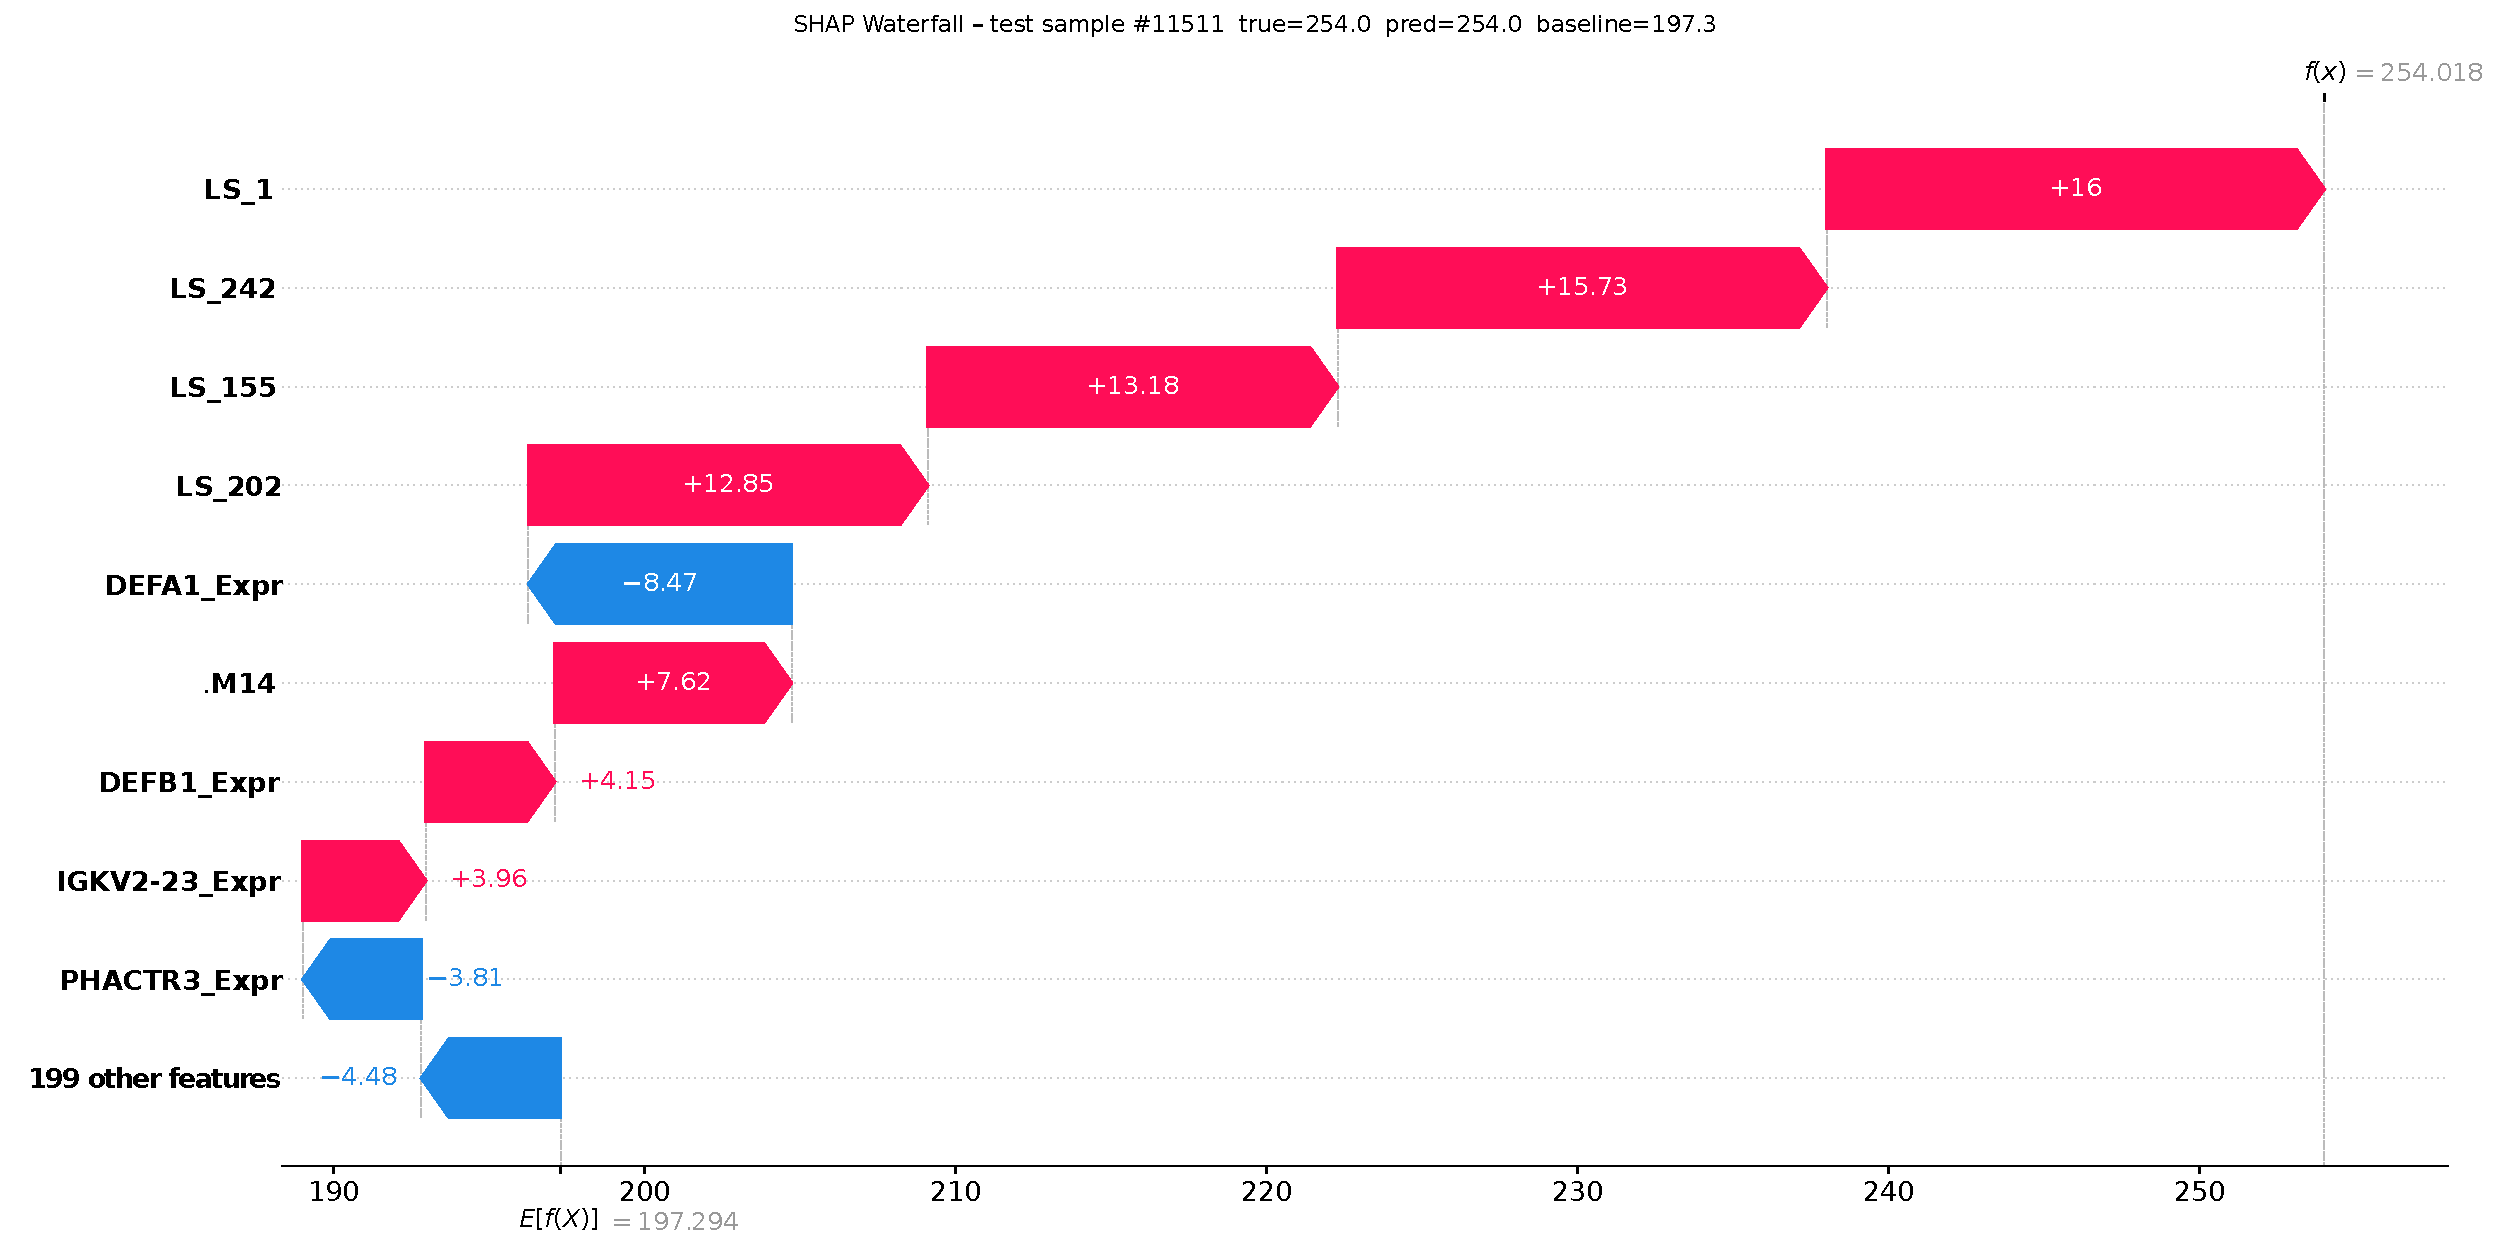
\includegraphics[width=\textwidth]{figures/SHAP_resistance_idx11511.pdf}
        \caption{Resistant: true AUC $= 254.0$, predicted $= 254.0$}
        \label{fig:shap_res}
    \end{subfigure}
    \caption{SHAP waterfall plots for individual test-set predictions from PREDICT-AML (TabPFN, KD-Embed). Starting from the base value ($\approx 197.3$), each bar shows the SHAP contribution of the top features pushing the final prediction higher (red, toward resistance) or lower (blue, toward sensitivity). (A)~Sensitive patient--drug pair (sample idx8432, true AUC $= 124.0$, predicted $= 124.0$): drug embedding dimensions LS\_125 ($\text{SHAP} = -24.4$) and LS\_214 ($-13.7$), together with patient feature \textit{POU4F1} expression ($-11.0$), drive the prediction well below baseline. (B)~Resistant patient--drug pair (sample idx11511, true AUC $= 254.0$, predicted $= 254.0$): drug embedding dimensions LS\_1 ($+16.0$) and LS\_242 ($+15.7$), together with LS\_155 ($+13.2$) and LS\_202 ($+12.8$), collectively push the prediction substantially above baseline, with \textit{DEFA1} expression ($-8.5$) providing a partially opposing effect. Waterfall plots for additional sensitivity and resistance examples are provided in Supplementary Figs.~8--9.}
    \label{fig:shap_individual}
\end{figure}

The waterfall plots reveal complementary interpretability patterns. In the sensitive prediction (Figure~\ref{fig:shap_sens}), particular drug embedding dimensions encode structural properties that favour cellular uptake or target engagement, while \textit{POU4F1} expression---a POU-domain transcription factor associated with differentiation state---further amplifies the drug's predicted effect. In the resistant prediction (Figure~\ref{fig:shap_res}), a distinct set of embedding dimensions dominates, reflecting the chemical basis for poor drug efficacy, with \textit{DEFA1} expression acting as a modest counterbalancing signal. Together, these results demonstrate that PREDICT-AML's predictions are driven by an interpretable combination of drug chemical properties and patient transcriptomic context, supporting its potential utility as a clinical decision support tool.

%%%%%%%%%%%%%%%%%%%%%%%%%%%%%%%%%%%%%%%%%%%%%
\section{Discussion}\label{sec4}
In this study, we present PREDICT-AML, a machine learning framework developed to accurately forecast patient-specific drug responses in AML using the richly annotated, multi-omics BeatAML dataset. Our work addresses critical limitations in earlier BeatAML studies by shifting from retrospective, correlative analyses to a predictive modeling approach capable of generalizing across unseen patients and, importantly, across independent external cohorts. The PREDICT-AML framework integrates diverse data modalities---gene expression, somatic mutation status, pathway activity, immune cell-state enrichment, and key clinical features---with four complementary drug molecular encodings.

\textbf{Patient-stratified CV as the honest clinical benchmark}: A central contribution of this work is the demonstration that standard random cross-validation significantly overestimates a model's real-world predictive utility in AML drug response prediction. TabPFN with MolFormer drug embeddings achieves $r_{pc} = 0.808$ under random CV but only $r_{pc} = 0.716$ under patient-stratified CV---a gap of approximately $13\%$ in Pearson correlation and $22\%$ in MAE. This inflation is not unique to one model or drug representation: across all four drug encodings, random CV consistently overstates performance by similar margins. The patient-stratified CV directly simulates clinical deployment, where predictions are made for new patients whose samples were never in the training set, and therefore represents the appropriate benchmark for reporting model performance. We recommend that future AML drug response prediction studies adopt patient-stratified evaluation as the primary metric.

\textbf{TabPFN as primary model}: A further contribution of this work is the adoption of TabPFN \cite{hollmann2023tabpfn} as the primary predictive architecture. Unlike gradient-boosted trees and neural networks that require dataset-specific optimization, TabPFN leverages meta-learned in-context learning to make accurate predictions in a single forward pass. The optimal patient-stratified CV result ($r_{pc} = 0.724 \pm 0.015$, MAE $= 31.054 \pm 0.742$; ablation configuration, KD-Embed) represents a substantial improvement over the best classical tree-based model, LightGBM (test $r_{pc} = 0.681$, MAE $= 38.399$; Table~\ref{table:benchmark_compact}). The drug-stratified CV result ($r_{pc} \approx 0.37$) provides an additional evaluation axis that quantifies generalization to structurally novel compounds---a challenge where chemical language models offer systematic advantages over simpler physicochemical encodings.

\textbf{Drug representation matters for novel-drug generalization}: Our results demonstrate that richer chemical language representations (ChemBERTa, MolFormer) offer a systematic advantage over simpler physicochemical descriptors or SMILES autoencoder embeddings specifically in the drug-stratified setting. The improvement in drug-stratified CV $r_{pc}$ from $0.306$ (Only\_PC) to $0.377$ (ChemBERTa) highlights the value of pre-training on large molecular databases to learn transferable chemical structure information. Under patient-stratified and random CV, differences between drug representations are small, suggesting that patient multi-omics features are the dominant predictors in those scenarios.

\textbf{Multi-cohort external validation}: To our knowledge, PREDICT-AML is the first AML drug response prediction framework validated simultaneously on two independent external cohorts spanning different measurement platforms (AUC vs.\ DSS), geographic sites (US vs.\ Finland), and patient population sizes. The LeeAML validation \cite{lee2018machine} confirms that transcriptomic and genomic signals predictive of drug sensitivity in BeatAML transfer to patients from a distinct US clinical center with differing treatment protocols. The FIMM-AML validation \cite{malani2022implementing} further demonstrates cross-platform consistency, with model-predicted AUC values showing meaningful rank correlation with DSS measurements despite systematic scale differences. Together, these validations strengthen confidence that PREDICT-AML captures generalizable biological signals rather than dataset-specific artifacts.

\textbf{Prediction uncertainty}: The CI analysis provides a practical tool for translating model outputs into clinical decisions. Predictions with narrow CIs can inform therapeutic selection with high confidence, while wide-CI predictions flag cases where experimental validation or additional data collection would be most valuable. This uncertainty-aware framework aligns with the broader movement toward responsible AI in clinical medicine.

\textbf{Comparison with related work}: A recent reanalysis of BeatAML by Karathanasis et al.\ \cite{karathanasis2024machine} employed ElasticNet models to predict drug response for 122 drugs (mean $r_{pc}$ of $0.36$). While demonstrating the predictive value of RNA-seq data, their linear modeling approach lacks the non-linear feature interaction capacity of PREDICT-AML. The MDREAM ensemble framework \cite{trac2023prediction} achieves strong performance on BeatAML but restricts evaluation to the 122 drugs with $> 100$ patient-drug pairs, inflating apparent test performance by excluding low-sample drugs. Unlike PREDICT-AML, MDREAM does not incorporate pathway proximity features or provide prediction uncertainty estimates. The Quadratic Phenotypic Optimization Platform (QPOP) \cite{sahib2024combinatorial} demonstrated high clinical accuracy (86.2\%) but relies on ex vivo drug combination experiments rather than in silico prediction, limiting its scalability. MSDRP \cite{zhao2023msdrp} integrates deep learning with cell line features but lacks direct validation in patient-derived datasets. PREDICT-AML uniquely combines broad model benchmarking, external multi-cohort validation, uncertainty quantification, and pathway-aware drug representation.

\textbf{Limitations}: Several important limitations warrant discussion. The BeatAML training set, while large by AML standards, may not represent the full demographic and geographic diversity of AML patients. The drug-stratified CV performance ($r_{pc} \approx 0.37$) indicates that predicting response to truly novel drugs remains challenging. The FIMM-AML cross-platform comparison is complicated by systematic differences between AUC and DSS metrics. Additionally, PREDICT-AML currently models drug response as a continuous variable; translating predictions to binary clinical outcomes (response/non-response) would require calibration against clinical endpoint data. Future work should incorporate single-cell transcriptomic data to model intra-patient heterogeneity, integrate longitudinal samples to track evolving drug sensitivity, and explore causal inference methods to improve biological interpretability.

%%%%%%%%%%%%%%%%%%%%%%%%%%%%%%%%%%%%%%%%%%%%%
\section{Conclusion}\label{sec5}
In this study, we developed PREDICT-AML, a machine learning framework for predicting personalized drug responses in acute myeloid leukemia patients. By leveraging the rich multi-omics and clinical data from the BeatAML cohort and extending validation to independent LeeAML and FIMM-AML cohorts, we demonstrate that transcriptomic, genomic, and pathway-based features carry generalizable drug sensitivity signals across patient populations and measurement platforms.

The optimal PREDICT-AML model, based on TabPFN with MolFormer drug embeddings, achieves a patient-stratified cross-validation Pearson correlation of $r_{pc} = 0.716$ (MAE $= 31.592$) on BeatAML---the clinically meaningful benchmark that evaluates generalization to previously unseen patients. Critically, we show that standard random cross-validation inflates this estimate to $r_{pc} = 0.808$, overstating generalization by $\sim\!13\%$; patient-stratified evaluation is the appropriate standard for reporting AML drug response prediction performance. Drug-stratified CV ($r_{pc} = 0.372$) further reveals where richer chemical language representations (ChemBERTa, MolFormer) provide systematic advantages over simpler physicochemical encodings. The framework also provides calibrated prediction uncertainty estimates, offering a practical tool for clinical decision support.

Further validation on prospective clinical cohorts and integration with single-cell data remain important future directions. The SHAP-based interpretability analysis presented in Section~\ref{sec3.7} identifies drug embedding dimensions and key transcriptomic features (e.g., \textit{CDC42BPA}, \textit{IGSF10}, \textit{CEACAM6}) as the primary drivers of predicted drug sensitivity, providing a mechanistically grounded basis for clinical interpretation. More comprehensive interpretability analyses using methods such as GroupShapley \cite{jullum2021groupshapley} could provide further insights by grouping related molecular features driving drug response predictions. In conclusion, PREDICT-AML represents a significant step toward precision medicine in AML treatment, with the potential to guide clinicians in selecting optimal therapies based on individual patient multi-omics profiles.

\section*{Declarations}

\bmhead{Ethics approval and consent to participate}
N/A

\bmhead{Consent for Publication}
All authors have read the manuscript and provide consent for publication.

\bmhead{Availability of Data and Material}
All code used to generate the workflow, along with a detailed step-by-step process to obtain the results and corresponding analysis, is provided at: \url{https://github.com/raghvendra5688/PT-AML}.

\bmhead{Competing interests}
The authors declare no competing interests.

\bmhead{Supplementary information}
Supplementary information relevant to the manuscript is aggregated and provided as an additional file.

\bmhead{Funding}
The authors thank the Qatar National Library (QNL) for their support in providing resources and funding the APC, which was instrumental in completing this research. All authors have consented to this acknowledgment.

\bmhead{Acknowledgements}
Open Access funding provided by the Qatar National Library.

\bmhead{Authors' Contributions}
R.M.\ and H.B.\ conceived the study. S.P.J.\ and R.M.\ collected, curated and assimilated the data. S.P.J.\ and R.M.\ performed the feature engineering. R.M.\ built the machine learning models and conducted external validation experiments. S.P.J.\ performed association analysis. S.P.J., H.B.\ and R.M.\ wrote and revised the manuscript. H.B.\ and R.M.\ supervised the study.

\bibliography{sn-bibliography}

\end{document}
